\RequirePackage{fix-cm}
%

%\documentclass{svjour3}                     % onecolumn (standard format)
\documentclass[smallcondensed]{svjour3}     % onecolumn (ditto)

%надо закомментировать следующую строку!
%\usepackage[top=3cm, bottom=3cm, right=5cm]{geometry} 

%\documentclass[smallextended]{svjour3}       % onecolumn (second format)
%\documentclass[twocolumn]{svjour3}          % twocolumn
%
\smartqed  % flush right qed marks, e.g. at end of proof
%
\usepackage{graphicx}
%
%\usepackage{mathptmx}      % use Times fonts if available on your TeX system
%
% insert here the call for the packages your document requires
%\usepackage{latexsym}
% etc.
%
% please place your own definitions here and don't use \def but
% \newcommand{}{}
%
% Insert the name of "your journal" with
\journalname{Journal of Global Optimization}
%
\begin{document}

%надо закомментировать следующую строку!
%\fontsize{12}{13pt}\selectfont 

\title{Solving a set of global optimization problems by the parallel technique with uniform convergence
%On the uniform convergance of Global Search Algorithm when solving in parallel a series of optimization problems
\thanks{This study was supported by the Russian Science Foundation, project No 16-11-10150.}
}

\titlerunning{Solving a set of global optimization problems}        % if too long for running head

\author{Konstantin Barkalov         \and
        Roman Strongin 
}

%\authorrunning{Short form of author list} % if too long for running head

\institute{K. Barkalov  \at
               Institute of Information Technology, Mathematics and Mechanics\\ Lobachevsky State University of Nizhni Novgorod\\ Nizhni Novgorod, Russia \\
              \email{konstantin.barkalov@itmm.unn.ru} 
           \and
           R. Strongin \at
					Institute of Information Technology, Mathematics and Mechanics\\ Lobachevsky State University of Nizhni Novgorod\\ Nizhni Novgorod, Russia \\
							\email{strongin@unn.ru} 
}

\date{Received: date / Accepted: date}
% The correct dates will be entered by the editor


\maketitle

\begin{abstract}

In this paper, we consider solving a set of global optimization problems in parallel. The proposed novel algorithm provides uniform convergence to the set of solutions for all problems treated simultaneously. The current accuracy for each particular solution is estimated by the difference in each coordinate from the point of global decision. The main statement is given in the corresponding theorem. For the sake of illustration some computational results with hundreds of multidimensional global problems are provided. 

%This paper considers solving a series of Lipschitz optimization problems in parallel. A novel algorithm has been proposed, which provides the convergence to the solutions to all problems in the series simultaneously, regardless of the particular form of the objective function in various problems. A uniform decrease of the distance between the optimizer and current estimate of this one in all problems is the main advantage of the proposed algorithm. A theorem on the uniform convergence of the algorithm has been proven. The results of the computational experiments carried out on several hundred global optimization problems of various dimensions are presented. 

\keywords{ global optimization \and Peano-type space filling curves \and uniform convergence \and parallel computing}

\end{abstract}

\section{Introduction} \label{intro}

This paper considers global optimization problems of the following form:
\begin{eqnarray}\label{main_problem}
& \varphi(y^\ast)=\min{\left\{\varphi(y):y\in D\right\}},\\
& D=\left\{y\in R^N: a_i\leq y_i \leq b_i, 1\leq i \leq N\right\}. \nonumber
\end{eqnarray}
The objective function is assumed to satisfy the Lipschitz condition 
\[
\left|\varphi(y')-\varphi(y'')\right|\leq L\left\|y'-y''\right\|,\; y',y'' \in D,\; 0<L<\infty,
\]
with the constant $L$ unknown a priori. The analytical form of the function may be unknown, i.e. the objective function may be defined by an algorithm for computing the function values within the search domain (a ``black-box'' function). At the same time, it is assumed that even a single computation of the objective function value may be a time-consuming operation since it involves numerical modeling when solving applied problems.

The assumption regarding the fulfillment of the Lipschitz condition for the objective function is typical of many approaches (see, for example \cite{Strongin2000}--\cite{Paulavicius2014}). In recent years, the theory and the methods for parallel Lipschitz global optimizations have been extensively developed. Parallel implementations have been proposed for many well-known algorithms \cite{Gergel2005}--\cite{Paulavicius2011}.

Usually, the methods of global optimization (both sequential and parallel) are intended to solve a single optimization problem. If one needs to solve a series of $q$ problems, the problems in the series are solved sequentially, one after another. Therefore, the optimum estimation in the $i$-th problem in the series remains undefined until all preceding problems of the series (with the indices $1, 2, ..., i-1$) have been completely solved. In the case of limited computational resources, the optima estimates in the problems $i+1,..., q$ will not be obtained if the computation resources are exhausted while solving the $i$-th problem.

Situations when a series of $q$ problems must be solved are not an extraordinary. For example, a series of scalar problems arises when one needs to find a Pareto set in solving multi-objective optimization problems. In this case, the solution of a single scalar problem corresponds to one of the Pareto optimal points of a multi-objective problem (for reference, a review of the scalarization techniques is presented in \cite{Ehrgott2005}). A series of optimization problems also arises when using dimension reduction methods to solve multidimensional optimization problems. It is known that a multidimensional problem can be reduced to a set of problems of lower dimension. A detailed description of various dimension reduction schemes is presented in \cite{Strongin2000,Sergeyev2013}. 
%A series of test problems can be obtained using some generator (see, for example, \cite{Gaviano2003}).

When solving a set of problems, it is useful to get the estimates of the optima for all the problems at once as early as possible. This may be necessary to evaluate the expedience of continuing the search process at any point in time. It is also desirable to have the estimates of optima for all problems with the same precision. Running several independent processes, each solving one of the problems in the series on a parallel computer system, has a number of disadvantages. First, a workload imbalance between the processors will occur. If solving the $i$-th problem requires considerably fewer iterations of the method than solving the $j$-th problem, the processor tasked with handling the $i$-th problem would remain idle after completing the task. Second, the estimates of the optima will be obtained with different precision in different problems. Simpler problems will be solved with higher precision, whereas precision will be lower for more complex problems. 

The goal of this study was to develop a method for solving a series of global optimization problems, which would be free of the drawbacks listed above. Namely, the method should ensure: 
\begin{itemize}
	\item a uniform load for all processors/cores employed;
	\item a uniform convergence to the solutions of all problems in the series.
\end{itemize} 
%new text begins
Here and below uniform convergence is taken to mean proportional decreasing of the distance between the best iteration point and the global optimizer in all the problems in the series.
%new text ends

The proposed method is a further development of the Global Search Algorithm (GSA) and of its parallel generalization described in detail in \cite{Sergeyev1994}--\cite{Barkalov2016} as well as in monographs \cite{Strongin2000,Sergeyev2013}.
%new text begins
GSA was developed in the framework of a stochastic model as a one-step optimal Bayesian method that distinguishes it from the methods optimal in the worst case (see, for example, \cite{Zilinskas2013}). The idea of average optimality of global optimization algorithms rests on the assumption (which is typical of applied problems) that the worst case objective function $\varphi=const$ is not very realistic.
%new text ends

The main part of this article is organized as follows. In Section 2, a description of the GSA is presented, and theoretical statements regarding its convergence are given. The modification of the algorithm that makes it applicable for solving a series of problems simultaneously is described in Section 3. A uniform convergence of the modified algorithm to solving a series of problems is substantiated in Section 4. Section 5 presents the results of the numerical experiments; a comparison is made of various parallelization methods between the processors when solving a series of multidimensional multiextremal test problems. Section 6 concludes the paper.

\section{Global search algorithm} \label{sec:1}

Let us consider a global optimization problem 
\begin{eqnarray}\label{stand_problem}
& \varphi(y^\ast)=\min{\left\{\varphi(y):y\in D\right\}},\\
& D=\left\{y\in R^N: -2^{-1}\leq y_i \leq 2^{-1}, 1\leq i \leq N\right\}, \nonumber
\end{eqnarray}
with a Lipschitzian objective function. The issues related to reducing more general problem statements to standard statement (\ref{stand_problem}) were considered in \cite{Strongin2009}.

Using a continuous unambiguous mapping $y(x)$ of the interval $[0,1]$ of the real axis onto hypercube $D$ from (\ref{stand_problem}) (\textit{Peano space-filling curve}) one can reduce the multidimensional problem (\ref{stand_problem}) to a one-dimensional problem
\begin{equation}\label{u_problem}
\varphi(y^\ast)=\varphi(y(x^\ast))=\min{\left\{\varphi(y(x)): x\in[0,1]\right\}}.
\end{equation}

As follows from the properties of the space-filling curve \cite{Strongin2000}, the reduced one-dimensional function $\varphi(y(x))$ satisfies a uniform H{\"o}lder condition
\[
\left|\varphi(y(x'))-\varphi(y(x''))\right|\leq H\left|x'-x''\right|^{1/N},
\]
where the H{\"o}lder constant $H$ is related to the Lipschitz constant $L$ by the relationship 
\begin{equation}\label{L_and_H}
H=2L\sqrt{N+3}.
\end{equation}
Problems of numerical construction of Peano-type space filling curves and the corresponding theory are considered in detail in \cite{Strongin2000,Sergeyev2013}. Here we will note that a numerically constructed curve (\textit{evolvent}) is $2^{-m}$ accurate approximation of the theoretical Peano curve in $L_\infty$ metric, where $m$ is an evolvent construction parameter. 

The algorithm considered here generates a series of preimages  $x^k\in[0,1], k=0,1,2,...$, in which first the images $y^k=y(x^k)$ and then the values of the objective function $z^k=\varphi(y^k), k=0, 1, 2, ...$,  are computed. Let us call the process of computing a function value (including the construction of the image $y^k=y(x^k)$) a \textit{trial}, and the pair $(x^k, z^k)$ the result of the trial. The set of pairs
\[
\omega_k=\left\{(x^i,z^i):0\leq i \leq k\right\},
\]
corresponding to the first $k$ terms of the sequence of preimages ${x^k}$ is the \textit{search information} accumulated by the algorithm within $k$ steps. 

According to the global search algorithm, the first two trials are executed at the points 
\[
y^0=y(0), y^1=y(1).
\]
The choice of the point $y^{k+1},k\geq 1,$  for the next $(k+1)$-th trial is defined by the following rules.


\begin{enumerate}
	\item 
	Renumber the inverse images of all the points from the trials already performed  
\begin{equation}\label{y_i}
y^0=y(x^0), y^1=y(x^1),...,y^k=y(x^k)
\end{equation}
by subscripts in the increasing order of their coordinates, i.e.
\begin{equation}\label{x_i}
0=x_0<x_1<\dots <x_k=1,
\end{equation}
and associate these with the values $z_i=\varphi(y(x_i)), 0\leq i \leq k,$  computed at these points.
\item
Compute the maximum absolute value of the first divided differences
\begin{equation}\label{mu}
\mu = \max_{1 \leq i \leq k}\frac{\left|z_i-z_{i-1}\right|}{\Delta_i},
\end{equation}
where $\Delta_i=\left(x_i-x_{i-1}\right)^{1/N}$. If $\mu = 0$, set $\mu = 1$.
\item
For each interval $(x_{i-1}, x_i), \; 1\leq i \leq k,$  calculate the value
\begin{equation}\label{R}
R(i)=r\mu\Delta_i+\frac{(z_i-z_{i-1})^2}{r\mu\Delta_i}-2(z_i+z_{i-1})
\end{equation}
called the \textit{characteristic} of the interval; the real number $r>1$ being the input parameter of the algorithm.
\item 
Select the interval $(x_{t-1},x_t)$ corresponding to the maximum characteristic
\begin{equation}\label{MaxR}
R(t)= \max_{1 \leq i \leq k}R(i).
\end{equation}
If there are several such intervals, choose the minimum number satisfying condition (\ref{MaxR}) as $t$.
\item
Assume
\begin{equation}\label{xk1}
x^{k+1} = \frac{x_t+x_{t-1}}{2} - \mathrm{sign}(z_t-z_{t-1})\frac{1}{2r}\left[\frac{\left|z_t-z_{t-1}\right|}{\mu}\right]^N
\end{equation}
as the inverse image for the next trial point, i.e. the next trial is to be carried out at the point $y^{k+1}=y(x^{k+1})$ from $D$.
\end{enumerate}

Rules (\ref{y_i})--(\ref{xk1}) describe the sequence of decision functions 
\[
x^{k+1}=G_k^r(x^0,...,x^k,z^0,...,z^k), \; k=1,2,...,
\]
generating the sequence of inverse images $x^k\in[0,1]$, $x^{k+1} \notin \left\{x^0,...,x^k\right\}$, and also the sequence of trial points $y^k\in D$, $y^{k+1} \notin \left\{y^0,...,y^k\right\}$. This infinite sequence of trials may be terminated by meeting the stopping condition
\[
\Delta_t < \epsilon,
\]
where $t$ is from (\ref{MaxR}), and $\epsilon>0$ is the predefined accuracy. We will use the value
\[
\varphi_k^\ast=\min_{0\leq i \leq k}\varphi(y^i)
\]
and the point 
\[
y_k^\ast=\arg \min_{0\leq i \leq k}\varphi(y^i)
\]
as the estimate of the optimum corresponding to the $k$-th step of the algorithm.

The conditions for convergence of the algorithm described above are formulated in the form of the following theorem from \cite{Strongin2000}.


\textbf{Theorem 1} (sufficient convergence conditions)

Let the point $\overline{y}$ be a limit point of the sequence $\left\{y^k\right\}$ generated by the rules of GSA while minimizing a Lipschitzian function $\varphi(y)$, $y \in D$, with the constant $L$. Then:
\begin{enumerate}
	\item 
	If side by side with $\overline{y}$ there exists another limit point $y'$ of the sequence $\left\{y^k\right\}$, then $\varphi (\overline{y}) = \varphi (y')$.
	\item
	For any  $z^k=\varphi(y^k) \geq \varphi(\overline{y})$.
	\item
	If at the some step of the search process the value $\mu$ from (\ref{mu}) satisfies the condition
\begin{equation}\label{217}
r \mu > 2^{3-1/N}L\sqrt{N+3},
\end{equation}
then $\overline{y}$ is a global minimizer of the function $\varphi (y)$ over $D$ and any global minimizer $y^\ast$ from (\ref{stand_problem}) is also a limit point of the sequence $\left\{y^k\right\}$.
\end{enumerate}

\textbf{Remark 1}. It follows from relationship (\ref{L_and_H}) between the Lipschitz and H{\"o}lder constants, as well as from condition (\ref{217}) of the Theorem, that for the convergence of the algorithm, parameter $r$ should satisfy the condition
\begin{equation}\label{218}
r > 2^{2-1/N}.
\end{equation}

\textbf{Remark 2}. Substantiation of the theorem is obtained by reducing to the contradiction with condition (\ref{MaxR}), i.e. by deriving the consequence that the subsequent trial will be carried out within an interval without the maximum characteristic.

The algorithm considered above is very flexible and allows an efficient parallelization. Let us assume a multiprocessor system with $p$ cores/processors to be at our disposal. The computational complexity of the objective function is one of the basic assumptions (see Introduction). The computations related to applying the algorithm's decision rules will play a role with negligible overhead costs. In this regard, the execution of $p$ search trials in parallel on different cores/processors within one iteration of the method would be the most efficient parallelization scheme. Thus the obtained parallel algorithm will consist of the following.

The first $p$ trials are executed at the points $x^0 = 0$, $x^1 = 1$ and at the arbitrary internal points $x^2, ..., x^{p-1}$ of the interval $(0,1)$. Let us assume $n \geq 1$  iterations of the method to be completed, in the course of which the trials in $k=k(n)$ points $x^i, 0 \leq i \leq k,$ have been executed. Then, the points $x^{k+1},...,x^{k+p}$  of the search trials for the next $(n+1)$-th iteration are determined according to the following rules. 

Steps 1--3 of the parallel algorithm repeat steps 1--3 of GSA completely.

4. Arrange characteristics  $R(i), 1 \leq i \leq k$, in decreasing order 
\begin{equation}\label{Rdec}
R(t_1)\geq R(t_2)\geq \dots \geq R(t_{k})
\end{equation}
and select $p$ largest characteristics with interval numbers $t_j, 1\leq j \leq p$.

5. Carry out new trials at points $x^{k+j}\in(x_{t_j-1},x_{t_j}), 1\leq j\leq p$, computed according to the formula
\[
x^{k+j} = \frac{x_{t_j}+x_{t_j-1}}{2} - \mathrm{sign}(z_{t_j}-z_{t_j-1})\frac{1}{2r}\left[\frac{\left|z_{t_j}-z_{t_j-1}\right|}{\mu}\right]^N.
\]

The algorithm stops if condition $\Delta_{t_j}<\epsilon$ is satisfied for at least one index $t_j, 1 \leq j \leq p$ ; here $\epsilon>0$ is the predefined accuracy.

The decision rules of the Parallel Global Search Algorithm (PGSA) allow the following interpretation (see \cite{Strongin2000}), according to which series (\ref{Rdec}) arranges the intervals $(x_{t-1},x_t), 1 \leq t \leq k,$ with respect to the decreasing probability of the localization of the global minimizer of the function $\varphi(y(x))$ in these intervals. Therefore, (as part of this interpretation) one can expect the next trial points to be chosen within the intervals with the largest probabilities at the current search step.

The theorem on the convergence of PGSA is a generalization of theorem 1, of which is also presented in \cite{Strongin2000}. In particular, it has been proven that the introduction of the parallelism described above does not produce limit points different from those in a purely sequential scheme. The results of the investigation of sequential and parallel algorithms (as well as their various modification) are presented in \cite{Sergeyev1994,Grishagin1997}.

As an example of the work of GSA and PGSA, let us consider the minimization of a two-dimensional function obtained using a GKLS generator \cite{Gaviano2003}. In Fig.~\ref{example} (a) and (b), the contour plots of the objective function are presented. Fig.~\ref{example} (a) also shows the points of 261 trials (261 iterations) performed by the sequential version of the method until the required accuracy $\epsilon=10^{-2}$ was achieved. In Fig.~\ref{example} (b) the points of 304 trials (76 iterations) performed by the parallel algorithm using 4 cores, i.e. at $p=4$, are shown. The points of the trials performed by the parallel algorithm which differ from the trial points of the sequential algorithm are marked by the '+' sign.

\begin{figure}
\begin{minipage}{0.5\linewidth}
\center{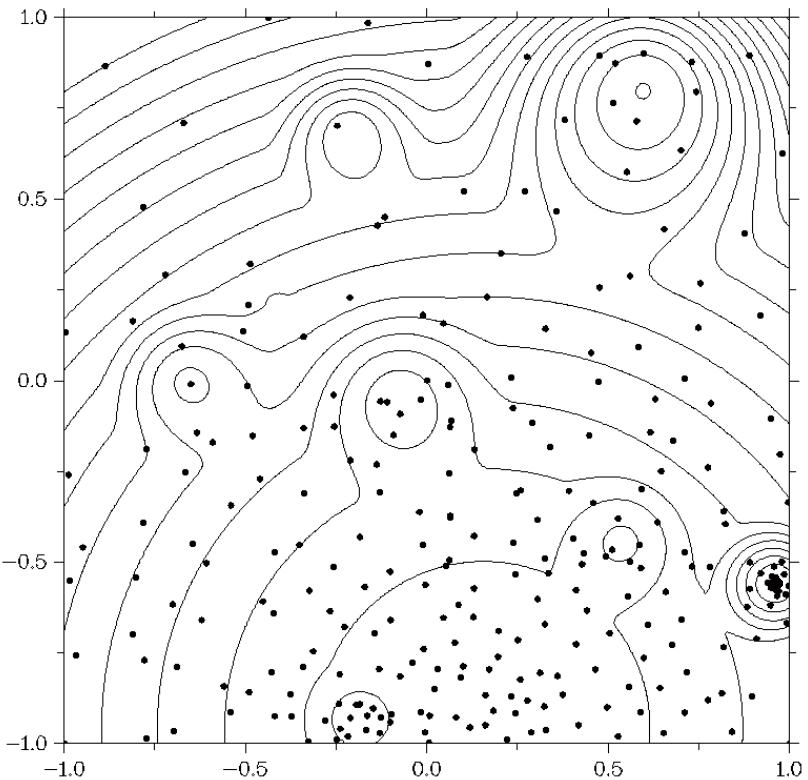
\includegraphics[width=1.0\linewidth]{fig2a.JPG} \\ (a)}
\end{minipage}
\hfill
\begin{minipage}{0.5\linewidth}
\center{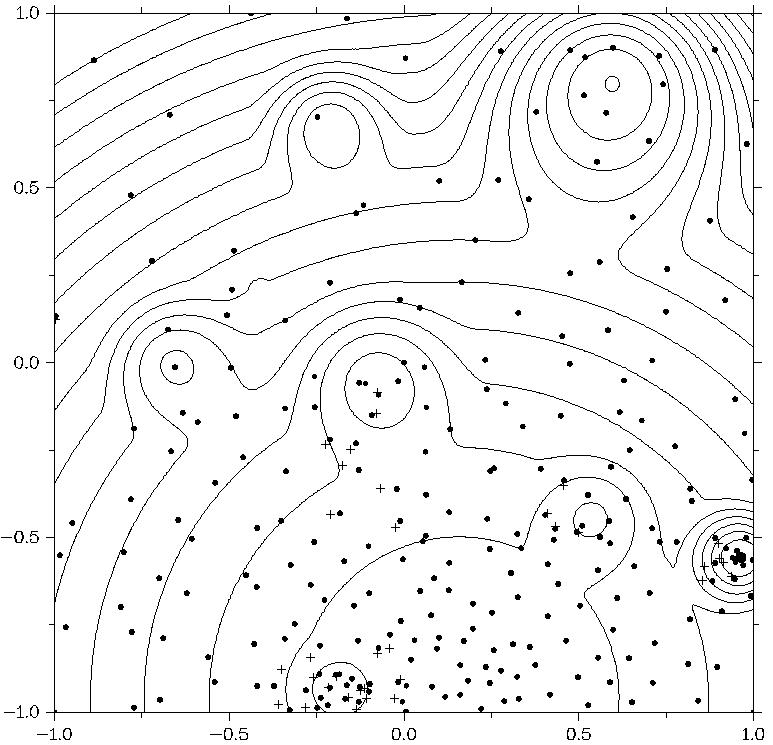
\includegraphics[width=1.0\linewidth]{fig2b.JPG} \\ (b)}
\end{minipage}
\caption{Solving a two-dimensional problem using (a) GSA and (b) PGSA}
\label{example}
\end{figure}


\section{An algorithm for solving a series of optimization problems} \label{sec:2}

Now, let us assume that we need to solve a series of $q$ problems 
\[
\min\left\{\varphi_1(y), y\in D \right\}, \min\left\{\varphi_2(y), y\in D\right\},..., \min\left\{\varphi_q(y), y\in D\right\}.
\]

It is necessary to introduce some modifications to the algorithm's computational scheme which would allow obtaining the estimates of optima in all the problems simultaneously. It is also necessary to provide the properties of the trial sequences generated during the minimization of different functions that do not depend on a particular form of the function.

The fulfillment of the inequality  
\begin{equation}\label{4phi}
R(j(l))>-4\varphi(y(x^\ast)),
\end{equation}
where $R(j(l))$ is the characteristic of the interval $(x_{j-1},x_j), \; j=j(l),$ containing the global minimizer $x^\ast$ of the function $\varphi(y(x))$ during the $l$-th iteration, is one of key properties used in \cite{Strongin2000} in the proof for the algorithm's convergence. 

As seen from the inequality (\ref{4phi}), the value of the characteristic of the interval $(x_{j-1},x_j), \; j=j(l),$ depends on the value of the function. If the algorithm is applied to minimize different functions, the values of the characteristics of intervals containing the global minimizer will be different as well. Hence in order to use the algorithm to minimize different functions, the algorithm's decision rules should be modified so that the value of the characteristic for the best interval does not depend on a particular form of the function. Let us consider such modifications.

1. If all characteristics $R(i)$ from (\ref{R}) at a given $k$ are divided by a quantity $r\mu$, where $\mu$ is from (\ref{mu}), i.e. if the characteristics are computed according to the formula
\[
R(i)=\Delta_i+\frac{(z_i-z_{i-1})^2}{(r\mu)^2\Delta_i}-\frac{2(z_i+z_{i-1})}{r\mu},
\]
the relationship of inequality between the characteristics would not change.

2. If a quantity $4\varphi_\ast^k/r\mu$  is added to all characteristics at a given $k$, the relationship of inequality between these would not change either.
Thus, the algorithms with characteristics (\ref{R}) and with characteristics
\begin{equation}\label{NewR}
R(i)=\Delta_i+\frac{(z_i-z_{i-1})^2}{(r\mu)^2\Delta_i}-\frac{2(z_i+z_{i-1}-2\varphi_\ast^k)}{r\mu}
\end{equation}
will generate the same sequences $\left\{x^k\right\}$. Consequently, the theorem of convergence is true for an algorithm with the characteristics (\ref{NewR}) since the normalization of the characteristics at each step does not change the relationship of their equality and superiority. Then, the inequality (\ref{4phi}) transforms into the inequality
\begin{equation}\label{zero}
R(j(l))>0,
\end{equation}
i.e. the lower bound for the best interval characteristic does not depend on the objective function now.

\section{Conditions of uniform convergence for the algorithm}

Let us consider the problems in the form  (\ref{stand_problem}) for a set of $q$ lipschitzian functions $\varphi_1(y), \varphi_2(y),...,\varphi_q(y)$ defined in $D$. Let us select (arbitrarily) two of these problems:
\begin{eqnarray} \label{two_problems}
\min\left\{\varphi(y), y\in D\right\}, \\ \nonumber
\min\left\{\psi(y), y\in D\right\}. \nonumber
\end{eqnarray}
Let us denote the characteristics (\ref{NewR}) for the first problem as $R_\varphi(i)$ and for the second problem as $R_\psi(j)$. Given that, 
\begin{eqnarray} \nonumber
R_\varphi(t_\varphi)= \max_{1 \leq i \leq k}R_\varphi(i), \\ \nonumber
R_\psi(t_\psi)= \max_{1 \leq j \leq s}R_\psi(j), \nonumber
\end{eqnarray}
where $k$ corresponds to the number of trials in the first problem and $s$ corresponds to the number of trials in the second one. The sequence of trials $\left\{v^k\right\}$ corresponds to the first problem and the sequence of trials $\left\{u^s\right\}$ corresponds to the second problem. The values $z^k=\varphi (y(v^k))$ correspond to the trial points $v^k\in [0,1]$ and the values $w^s=\psi(y(u^s))$ correspond to the trial points $u^s \in [0,1]$.

Let us consider the case where these two problems are solved simultaneously, and the selection of the interval $(v_{t_\varphi-1},v_{t_\varphi})$ or $(u_{t_\psi-1},u_{t_\psi})$ to execute the trials is determined by the condition
\begin{equation}\label{NewMaxR}
R(t)=\max\{R_\varphi(t_\varphi),R_\psi(t_\psi)\}.
\end{equation}

\textbf{Theorem 2} (on the convergence conditions)

Let the conditions for theorem 1 be satisfied for each problem (\ref{two_problems}) separately. 
Then solving both problems by the algorithm defining the interval for each next trial according to rule (\ref{NewMaxR}) for characteristics (\ref{NewR}) will generate two infinite sequences $\left\{v^k\right\}$ and $\left\{u^s\right\}$, for the limit points of which theorem 1 is also true.

\textbf{Proof}. Let $l=k+s,l=0,1,2,...,$ and the condition $v^0=u^0=0$, $v^1=u^1=1$ be satisfied. Then, the sequence of trials (i.e. $\left\{y(v^k)\right\}$) will be infinite at least for one of the functions (let it be $\varphi(y)$), and theorem 1 will be true for this function. We show that the algorithm generates an infinite sequence $\left\{y(u^s)\right\}$ for the second function $\psi(y)$ as well, for which, consequently, theorem 1 is  also true.

Let the limit point $\overline{v}\in[v_{i-1},v_i]$ where $i=i(k)$ and the parameter of algorithm $r$ satisfies the condition $r>2^{2-1/N}$, according to (\ref{218}). From (\ref{mu})
\[
\mu_\varphi^2 \geq \left(\frac{|z_i-z_{i-1}|}{\Delta_i}\right)^2
\]
and, consequently,
\[
\frac{(z_i-z_{i-1})^2}{r^2\mu_\varphi^2\Delta_i}=\frac{(z_i-z_{i-1})^2\Delta_i}{(r\mu_\varphi\Delta_i)^2}\leq\frac{\Delta_i}{r^2}.
\]
Hence, according to (\ref{NewR})
\[
R_\varphi(i) \leq \Delta_i\left(1+\frac{1}{r^2}\right)-\frac{2(z_i+z_{i-1}-2\varphi_\ast^k)}{r\mu_\varphi}.
\]
Because $\overline{v}$ is the limit point of the sequence of preimages $\left\{v^k\right\}$ and $\varphi_\ast^k \geq \varphi(y(\overline{v}))$ at $k\rightarrow\infty$
\begin{eqnarray} \nonumber
\Delta_i\rightarrow 0, \\ \nonumber
z_i+z_{i-1}-2\varphi_\ast^k\rightarrow 0. \nonumber
\end{eqnarray}
Therefore, for any small $\delta>0$ there exists a large value of $k$ such that 
\begin{equation}\label{Rleqdelta}
R_\varphi(i)<\delta.
\end{equation}

Let $\psi_\ast^s=w_{j-1}$, i.e. the current minimum value of function $\psi(y)$ is achieved at the left point of the interval $(w_{j-1},w_j)$. Then 
\[
\frac{w_j+w_{j-1}-2\psi_\ast^s}{r\mu_\psi}=\frac{w_j-w_{j-1}}{r\mu_\psi} = \frac{\Delta_j(w_j-w_{j-1})}{r\mu_\psi \Delta_j}\leq \frac{\Delta_j}{r}
\]
and, taking into account that $r>2^{2-1/N}>2$,
\[
R_\psi(j)=\Delta_j+\frac{(w_j-w_{j-1})^2}{r^2\mu_\psi^2\Delta_j}-\frac{2(w_j+w_{j-1}-2\psi_\ast^s)}{r\mu_\psi} \geq \Delta_j\left(1-\frac{2}{r}\right) > 0.
\]
Hence, according to (\ref{Rleqdelta}), the inequality 
\[
R_\psi(j) > R_\varphi(i).
\]
will be true at large enough values of $k$, and the scheduled iteration falls into the interval $(u_{j-1},u_j)$, i.e. the sequence $\left\{u^s\right\}$ will be infinite as well.

\textbf{Theorem 3} (on the uniform convergence)

Let the conditions of theorem 2 be satisfied. Then the convergence to the limit points of the sequences $\left\{v^k\right\}$ and $\left\{u^s\right\}$ is uniform,
%new text begins
i.e. for any step $l=k+s$  the minimum distance between the points of the sequence $\left\{v^k\right\}$ and its limit point does not exceed a similar value for the sequence $\left\{u^s\right\}$. 
%new text ends

\textbf{Proof}. Let $v^\ast$ be the preimage of the global optimizer of the function $\varphi(y)$, and $u^\ast$ be the preimage of the global optimizer of the function $\psi(y)$, given that 
\[
v^\ast \in \left[v_{i-1},v_i\right], \; u^\ast \in \left[u_{j-1},u_j\right],
\]
and let 
\begin{equation}\label{RpsileqRphi}
R_\psi(j) > R_\varphi(i)
\end{equation}
at some step $l=k+s$. Consequently, the next trial will fall into the interval $(u_{j-1},u_j)$ before the interval $(v_{i-1},v_i)$. At large enough values of $s$, it follows from the convergence of $\left\{u^s\right\}$ to $u^\ast$ that $\psi_\ast^s=w_{j-1}$, whence 
\[
w_j+w_{j-1}-2\psi_\ast^s=w_j+w_{j-1}-2w_{j-1}=w_j-w_{j-1}
\]
and
\begin{equation}\label{Rpsij}
R_\psi(j) =\Delta_j+\Delta_j\left(\frac{w_j-w_{j-1}}{r\mu_\psi\Delta_j}\right)^2-2\Delta_j\frac{w_j-w_{j-1}}{r\mu_\psi\Delta_j}=\Delta_j\left(1-\frac{w_j-w_{j-1}}{r\mu_\psi\Delta_j}\right)^2,
\end{equation}
where $\Delta_j=(u_j-u_{j-1})^{1/N}$. Analogously, if $\varphi_\ast^k=z_{i-1}$, then
\begin{equation}\label{Rphii}
R_\varphi(i) = \Delta_i\left(1-\frac{z_i-z_{i-1}}{r\mu_\varphi\Delta_i}\right)^2,
\end{equation}
where $\Delta_i=(v_i-v_{i-1})^{1/N}$. Now, it follows from (\ref{RpsileqRphi})--(\ref{Rphii}) that
\[
\Delta_j\left(1-\frac{w_j-w_{j-1}}{r\mu_\psi\Delta_j}\right)^2 > \Delta_i\left(1-\frac{z_i-z_{i-1}}{r\mu_\varphi\Delta_i}\right)^2
\]
and
\[
\frac{\Delta_i}{\Delta_j} <  \frac{\left(1-\frac{w_j-w_{j-1}}{r\mu_\psi\Delta_j}\right)^2}{\left(1-\frac{z_i-z_{i-1}}{r\mu_\varphi\Delta_i}\right)^2}.
\]
Because 
\[
0 \leq \left|\frac{w_j-w_{j-1}}{r\mu_\psi\Delta_j}\right| \leq \frac{1}{r}, \; 0 \leq \left|\frac{z_i-z_{i-1}}{r\mu_\varphi\Delta_i}\right| \leq \frac{1}{r},
\]
then
\[
\frac{\Delta_i}{\Delta_j} <  \frac{\left(1+\frac{1}{r}\right)^2}{\left(1-\frac{1}{r}\right)^2}=\left(\frac{r+1}{r-1}\right)^2.
\]

Thus, at the moment when the next trial falls into the interval $(u_{j-1},u_j)$, the length of the interval $(v_{i-1},v_i)$ cannot exceed the length of the interval $(u_{j-1},u_j)$ by more than $\left(\frac{r+1}{r-1}\right)^2$ times. The uniform convergence has been proven.

\textbf{Remark 3}. It follows from the properties of the evolvent (see \cite{Sergeyev2013}) that any two close points $x',x''\in (0,1)$ correspond to close images $y'=y(x')$, $y''=y(x'')$ in the hypercube $D$, and if
\[
\left|x'-x''\right|\leq 2^{-N(m+1)},
\]
where $m\geq 1$, then
\[
\max \left\{  \left|y'_i-y''_i\right|: 1\leq i \leq N \right\} \leq 2^{-m}.
\]
Thus, the uniform convergence of the images in the multidimensional space also follows from the uniform convergence of the preimages on the one-dimensional interval as well.

\textbf{Remark 4}. Since two problems (\ref{two_problems}) were selected from a set of problems being solved arbitrarily, theorem 2 and theorem 3 will also be true for any pair of problems from the set being solved. At the same time, theorem 2 and theorem 3 will also be true for $q>2$ problems 
\[
\min\left\{\varphi_1(y), y\in D \right\}, \; \min\left\{\varphi_2(y), y\in D\right\},..., \; \min\left\{\varphi_q(y), y\in D\right\}
\]
being solved simultaneously by induction.

\textbf{Remark 5}. The theorems on uniform convergence for the parallel algorithm are proved similarly, which allows applying the multiprocessor systems to solve a set of problems simultaneously.

\textbf{Remark 6}. The parallel algorithm will provide a uniform workload distribution for the cores/processors used. We assume that computing the objective function value will be a time-consuming operation, and it accounts for the majority of the computation costs as compared to the application of the parallel algorithm decision rules (the computing and arrangement of the characteristics, the information interchange between parallel processes, etc.). However, just this most computationally costly part is parallelized ($p$ trials are executed at each iteration where $p$ is the number of cores/processors employed). Therefore, the load on the computer system will be close to its full capacity.


\section{Results of experiments}

One of the well-known approaches to investigating and comparing multiextremal optimization algorithms is based on the application of these methods for solving a set of test problems selected randomly from some constructed class. In this case, each test problem can be considered as a particular realization of a random function defined by means of a special generator. The application of multiextremal optimization algorithms to sets of these functions allows the efficiency of each particular algorithm to be evaluated.

The numerical comparison of the algorithms has been carried out using the GKLS test problem generator \cite{Gaviano2003}. This generator allows multiextremal optimization problems to be generated with known properties (the number of local minima, the size of their domains of attraction, the global minimizer, etc.). Eight GKLS classes of differentiable test functions of the dimensions $N = 2,3,4,$ and $5$ have been used. For each dimension, both \textit{Hard} and \textit{Simple} classes have been considered. The difficulty of a class was increased either by decreasing the radius of the attraction region of the global minimizer, or by decreasing the distance from the global minimizer $y^\ast$ to the domain boundaries. The global minimizer $y^\ast$ was considered to be found, if the algorithm generated a trial point $y^k$ in the vicinity of the global minimum, i.e. $\left|y^k-y^\ast\right| < \delta \left\|b-a\right\|$, where $\delta = 0.01$, $a$ and $b$ are the boundaries of the search domain $D$. When using the Global Search Algorithm, the parameter $r$ was set to $5$, the evolvent construction parameter was fixed as $m = 10$. The maximum allowable number of iterations per problem was $K_{max} = 10^6$.

Each series of problems was solved using a scheme to distribute the problems between the parallel threads ($S1$) and using the proposed scheme to simultaneously solve all problems ($S2$). The number of employed parallel threads $p$ was varied from $1$ to $24$.

The average numbers of trials executed by the algorithm depending on the number of threads when solving \textit{Simple} and \textit{Hard} classes of problems are presented in Tables \ref{tab:1} and \ref{tab:2}, respectively. The results demonstrate that both schemes of problem distribution between threads require an almost equal number of trials. The workload of each thread is also the same. In particular, there is an exact match between the number of trials for the sequential runs (at $p = 1$).  

\begin{table}
	\caption{Average number of iterations for the \textit{Simple} class}
	\label{tab:1}
	\center
	\begin{tabular}{cccccccccccc}
		\hline\noalign{\smallskip}
		$p$ & \multicolumn{2}{c}{ $N=2$ } & & \multicolumn{2}{c}{$N=3$} & & \multicolumn{2}{c}{$N=4$} & & \multicolumn{2}{c}{$N=5$}  \\
		\noalign{\smallskip} \cline{2-3} \cline{5-6} \cline{8-9} \cline{11-12}  \noalign{\smallskip}
		 & $S1$ & $S2$ & & $S1$ & $S2$ & & $S1$ & $S2$ & & $S1$ & $S2$  \\
		\noalign{\smallskip} \hline \noalign{\smallskip}
1	&	408	&	408	&	&	2502	&	2502	&	&	28254	&	28254	&	&	87261	&	87261	\\
2	&	408	&	415	&	&	2502	&	2496	&	&	28254	&	27206	&	&	87261	&	85994	\\
4	&	408	&	405	&	&	2502	&	2430	&	&	28254	&	30121	&	&	87261	&	78064	\\
8	&	408	&	402	&	&	2502	&	2505	&	&	28254	&	28980	&	&	87261	&	84337	\\
16	&	408	&	415	&	&	2502	&	2501	&	&	28254	&	28206	&	&	87261	&	82564	\\
24	&	408	&	400	&	&	2502	&	2416	&	&	28254	&	27868	&	&	87261	&	86252	\\
		\noalign{\smallskip}\hline
	\end{tabular}
\end{table}


\begin{table}
	\caption{Average number of iterations for the \textit{Hard} class}
	\label{tab:2}
	\center
	\begin{tabular}{cccccccccccc}
		\hline\noalign{\smallskip}
		$p$ & \multicolumn{2}{c}{ $N=2$ } & & \multicolumn{2}{c}{$N=3$} & & \multicolumn{2}{c}{$N=4$} & & \multicolumn{2}{c}{$N=5$}  \\
		\noalign{\smallskip} \cline{2-3} \cline{5-6} \cline{8-9} \cline{11-12}  \noalign{\smallskip}
		 & $S1$ & $S2$ & & $S1$ & $S2$ & & $S1$ & $S2$ & & $S1$ & $S2$  \\
		\noalign{\smallskip} \hline \noalign{\smallskip}
1	&	806	&	806	&	&	3873	&	3873	&	&	60972	&	60972	&	&	162475	&	162475	\\
2	&	806	&	807	&	&	3873	&	4104	&	&	60972	&	58382	&	&	162475	&	167728	\\
4	&	806	&	823	&	&	3873	&	4081	&	&	60972	&	57285	&	&	162475	&	172522	\\
8	&	806	&	881	&	&	3873	&	4153	&	&	60972	&	55353	&	&	162475	&	173725	\\
16	&	806	&	854	&	&	3873	&	4165	&	&	60972	&	60158	&	&	162475	&	178130	\\
24	&	806	&	887	&	&	3873	&	4270	&	&	60972	&	55939	&	&	162475	&	182821	\\
		\noalign{\smallskip}\hline
	\end{tabular}
\end{table}


In order to demonstrate the presence of the uniform convergence of the proposed algorithm for solving a series of problems, let us plot the functions $D_{av}(K)$ and $D_{max}(K)$ featuring the average and maximum deviation of the current approximation from the exact solution over all problems, depending on the total number of trials. 
Figs.~\ref{fig_last1},~\ref{fig_last2},~\ref{fig_last3} and \ref{fig_last4} show these functions plotted while solving five-dimensional \textit{Simple} class problems using a sequential algorithm and a parallel algorithm.
The number of trials is plotted on the abscissa (in millions) against the deviation of the current approximation from the exact solution of the problem on the ordinate. The red curve shows the first scheme of problem distributions while the green curve represents the second scheme. 

\begin{figure}
\begin{minipage}{0.5\linewidth}
\center{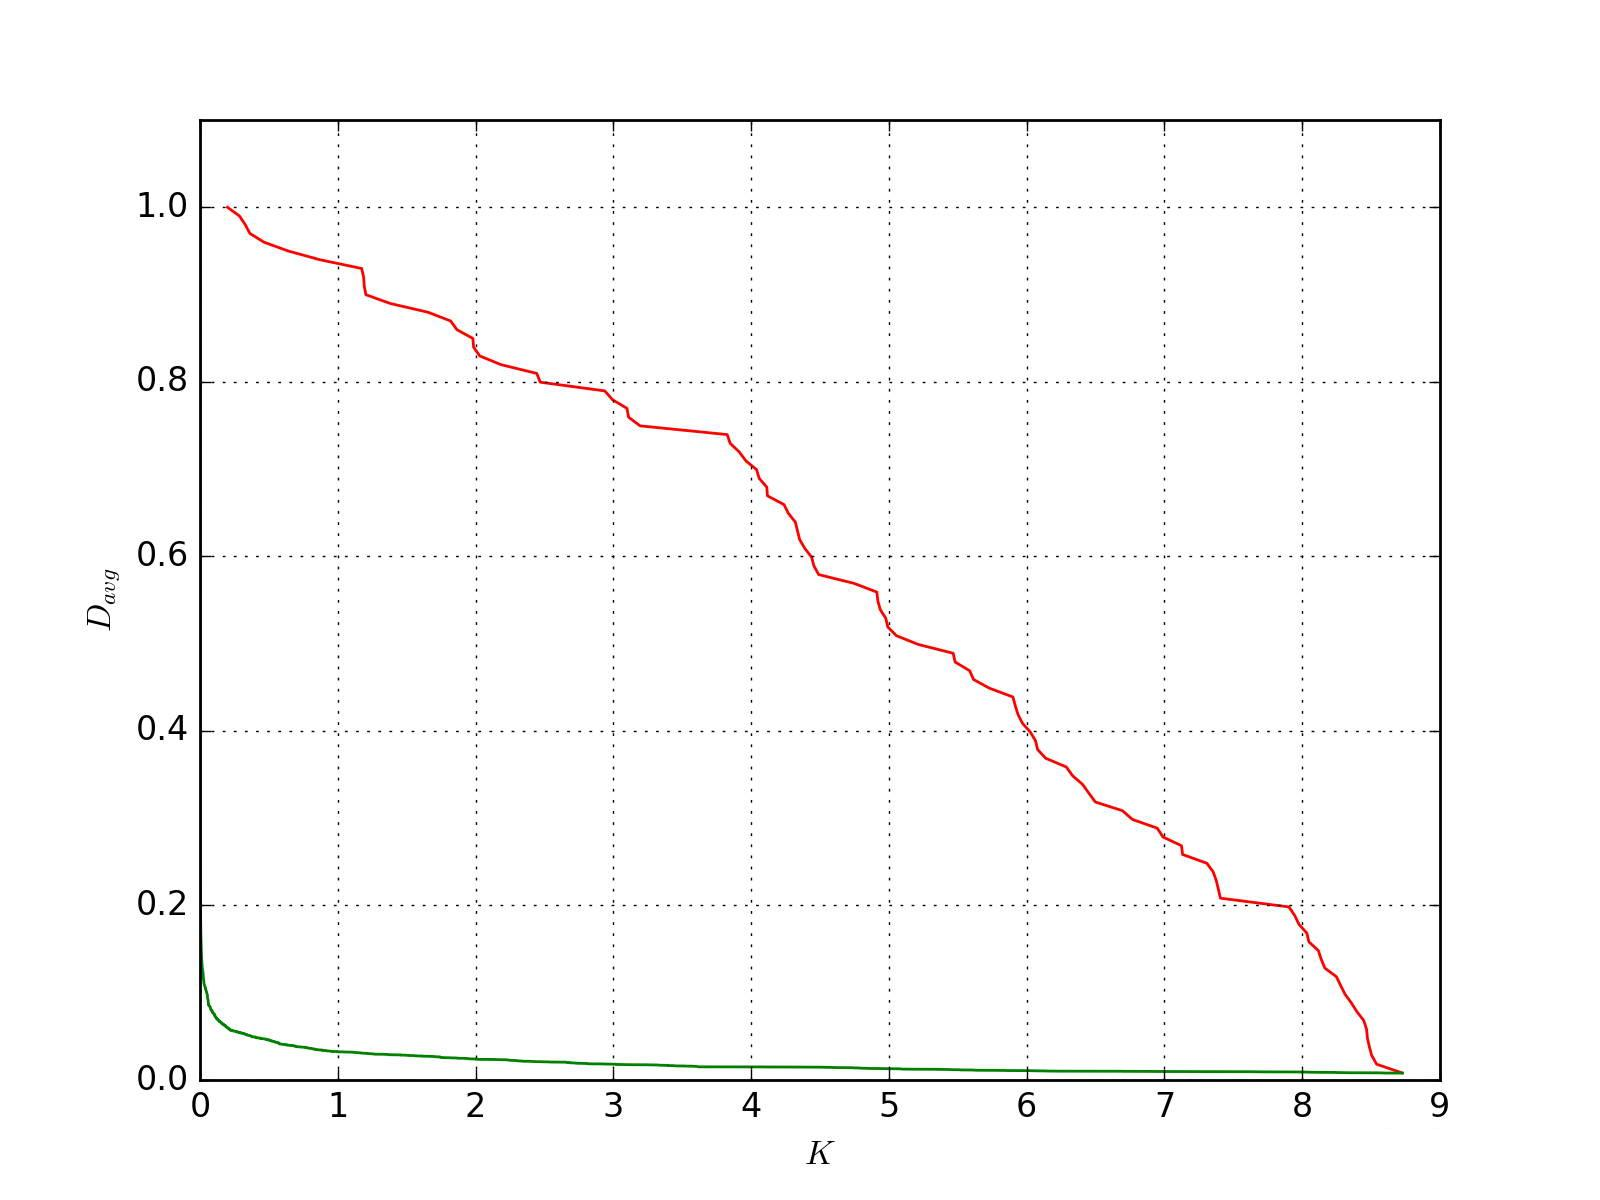
\includegraphics[width=1.0\linewidth]{fig3a.jpg} \\ (a)}
\end{minipage}
\hfill
\begin{minipage}{0.5\linewidth}
\center{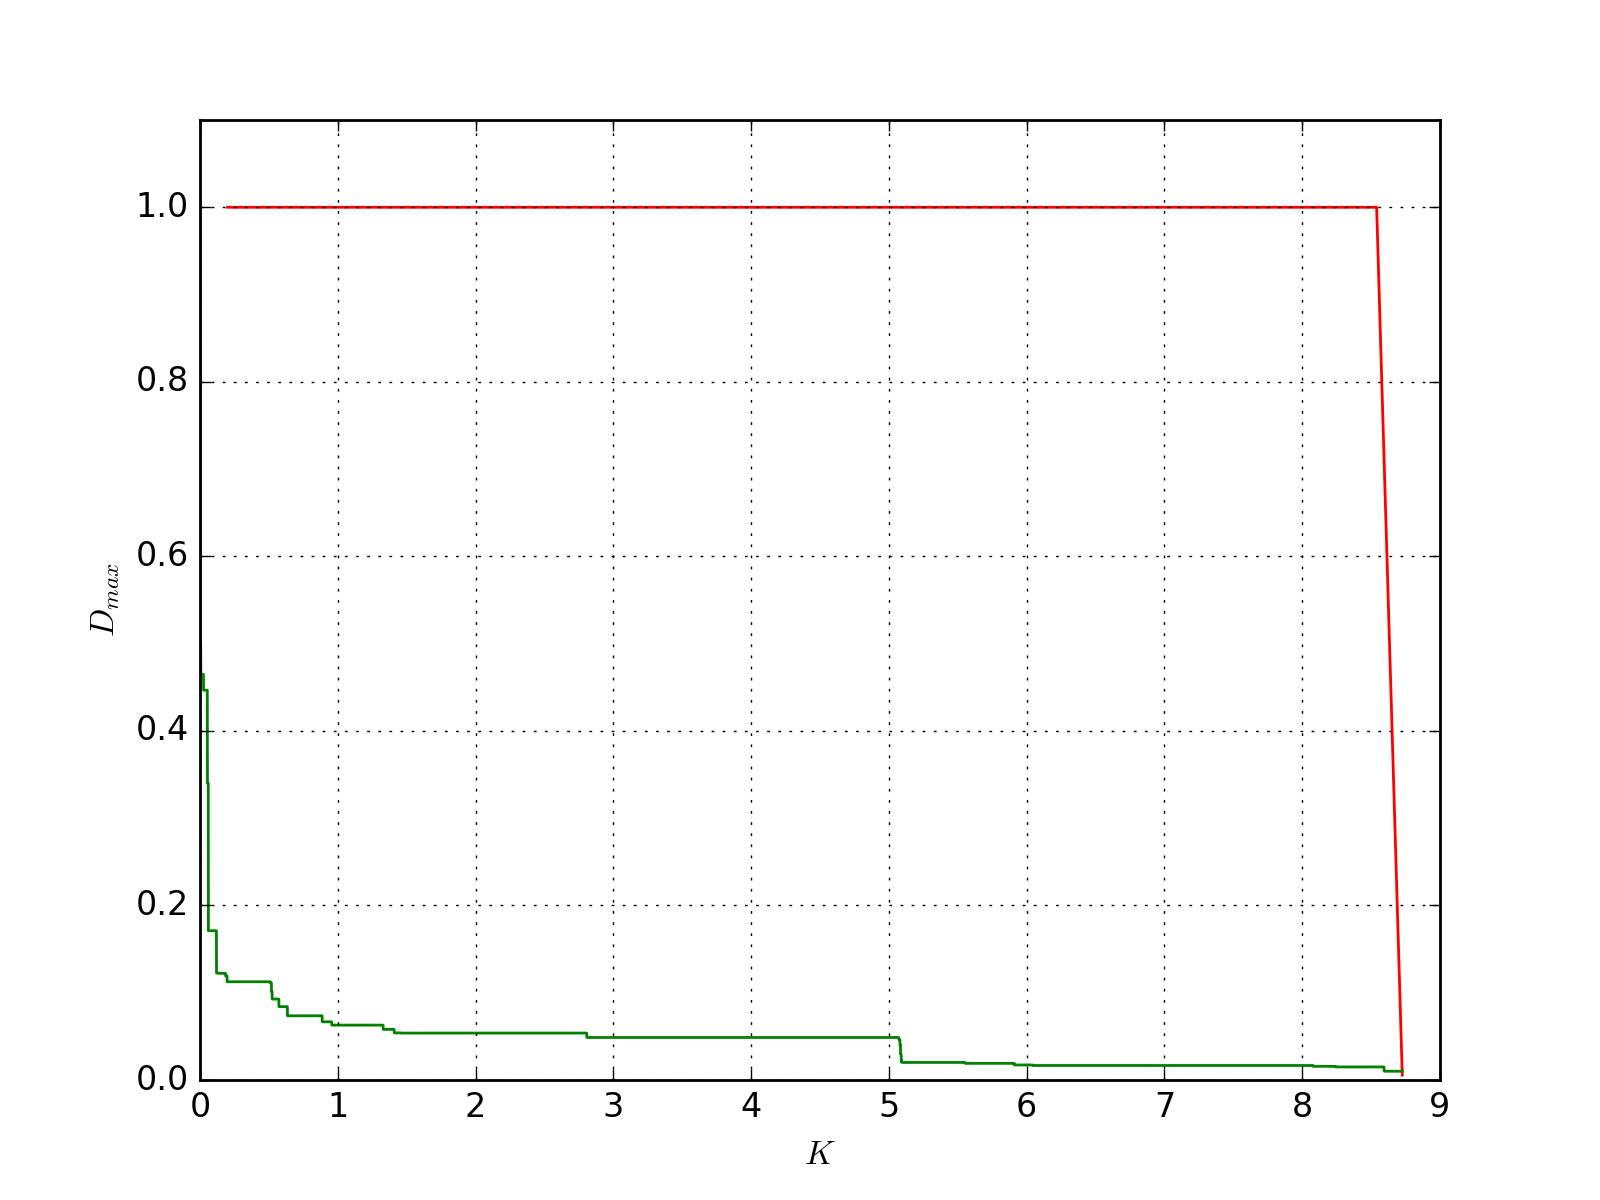
\includegraphics[width=1.0\linewidth]{fig3b.jpg} \\ (b)}
\end{minipage}
\caption{Average (a) and maximum (b) deviation of the current approximation from the exact solution for the sequential algorithm.}
\label{fig_last1}
\end{figure}

\begin{figure}
\begin{minipage}{0.5\linewidth}
\center{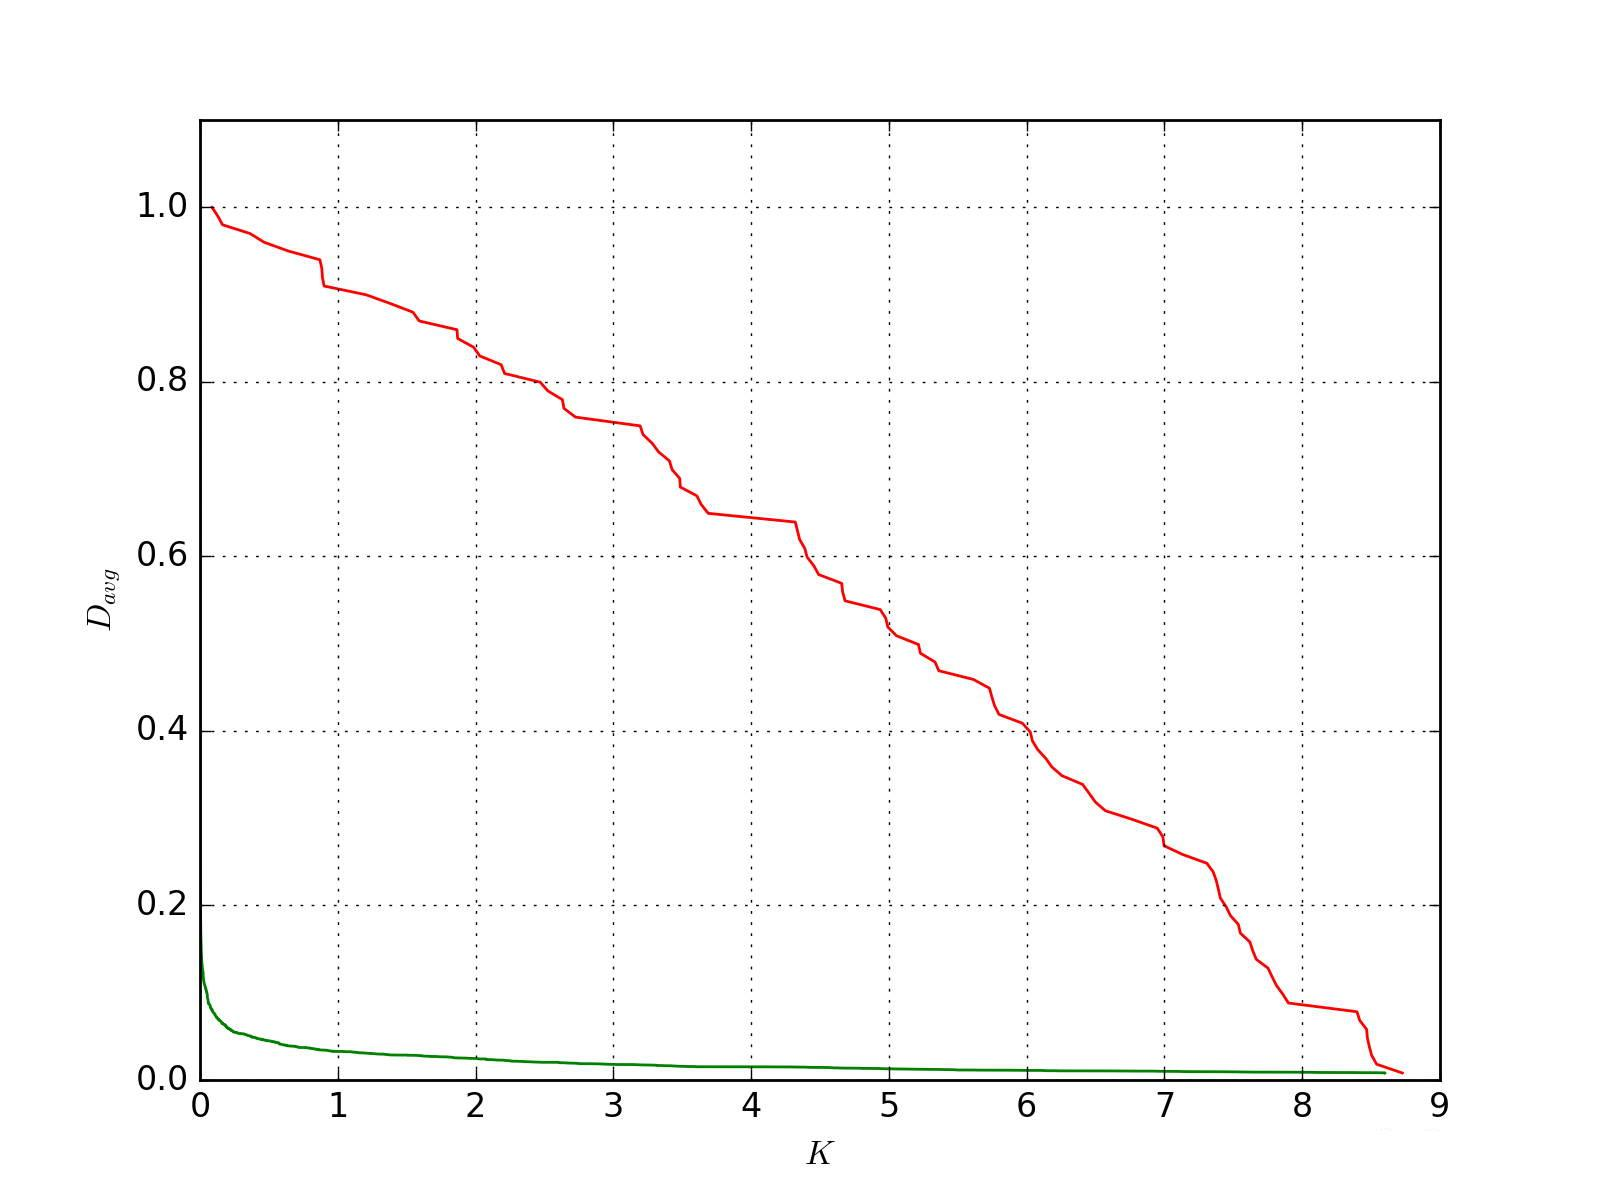
\includegraphics[width=1.0\linewidth]{fig4a.jpg} \\ (a)}
\end{minipage}
\hfill
\begin{minipage}{0.5\linewidth}
\center{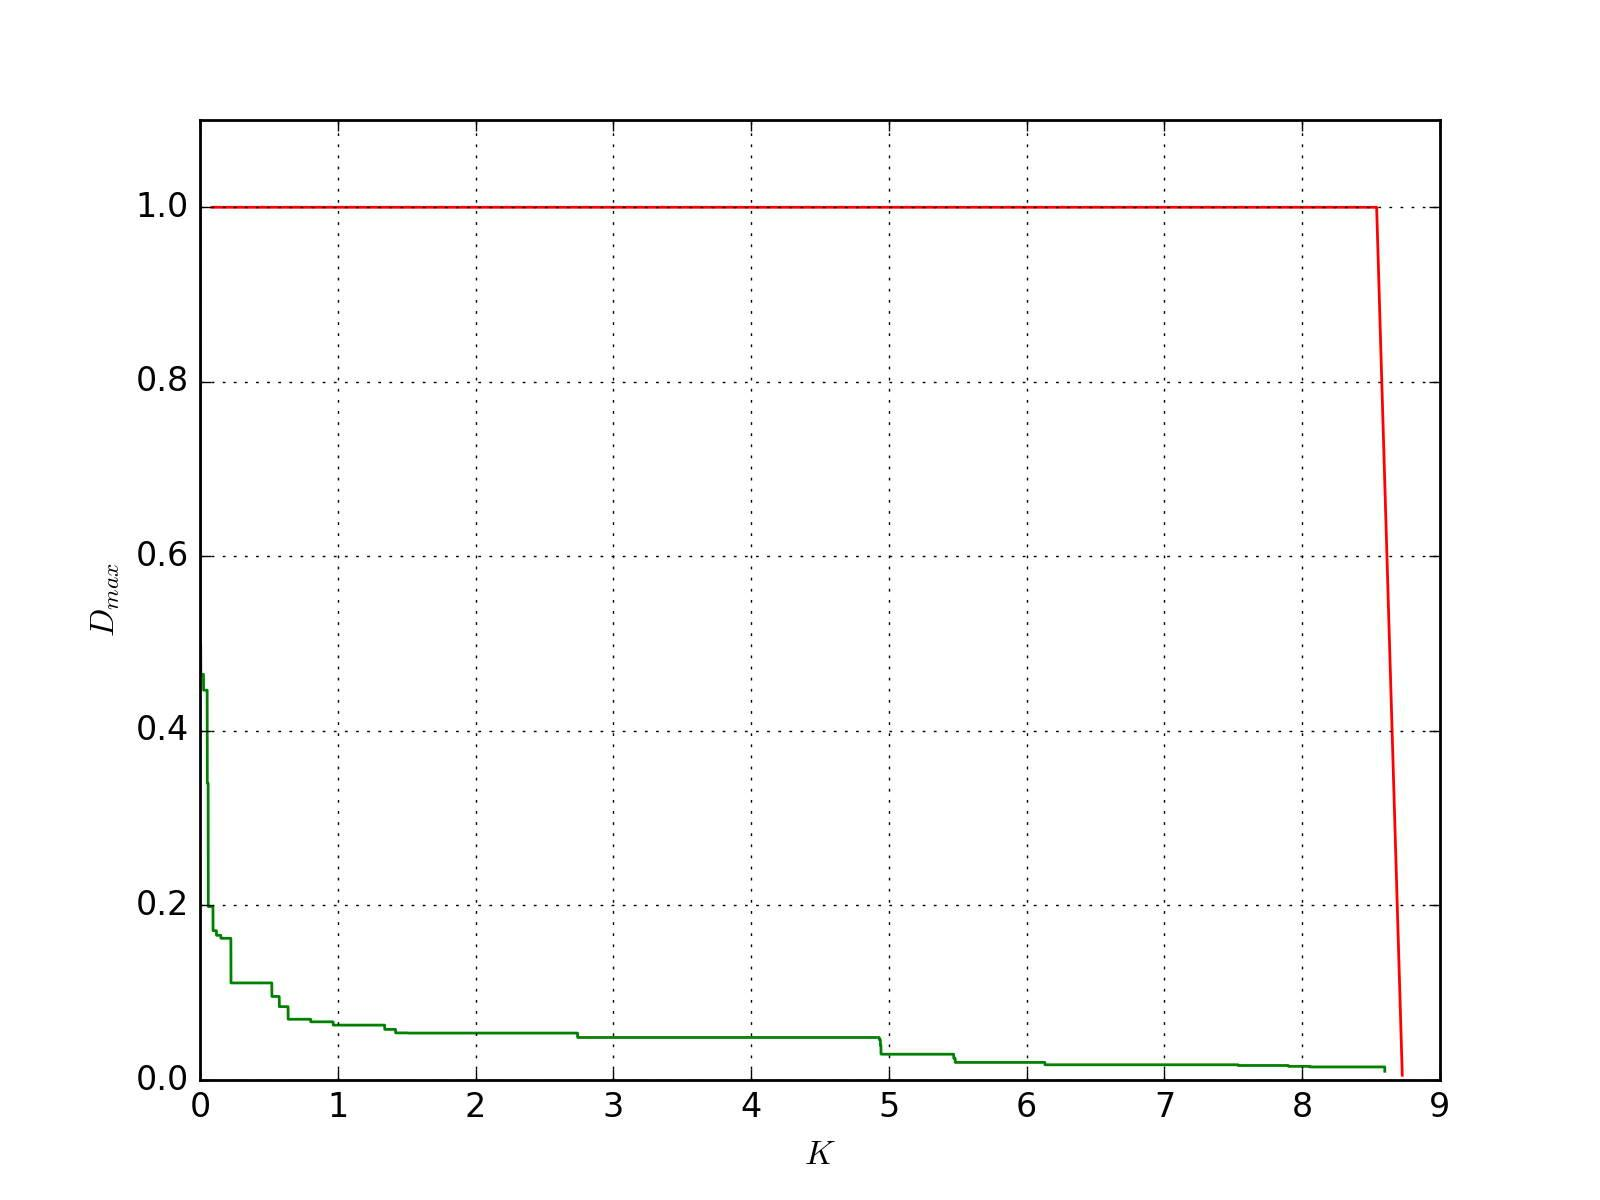
\includegraphics[width=1.0\linewidth]{fig4b.jpg} \\ (b)}
\end{minipage}
\caption{Average (a) and maximum (b) deviation of the current approximation from the exact solution for the parallel algorithm; the number of threads $p = 2$.}
\label{fig_last2}
\end{figure}


\begin{figure}
\begin{minipage}{0.5\linewidth}
\center{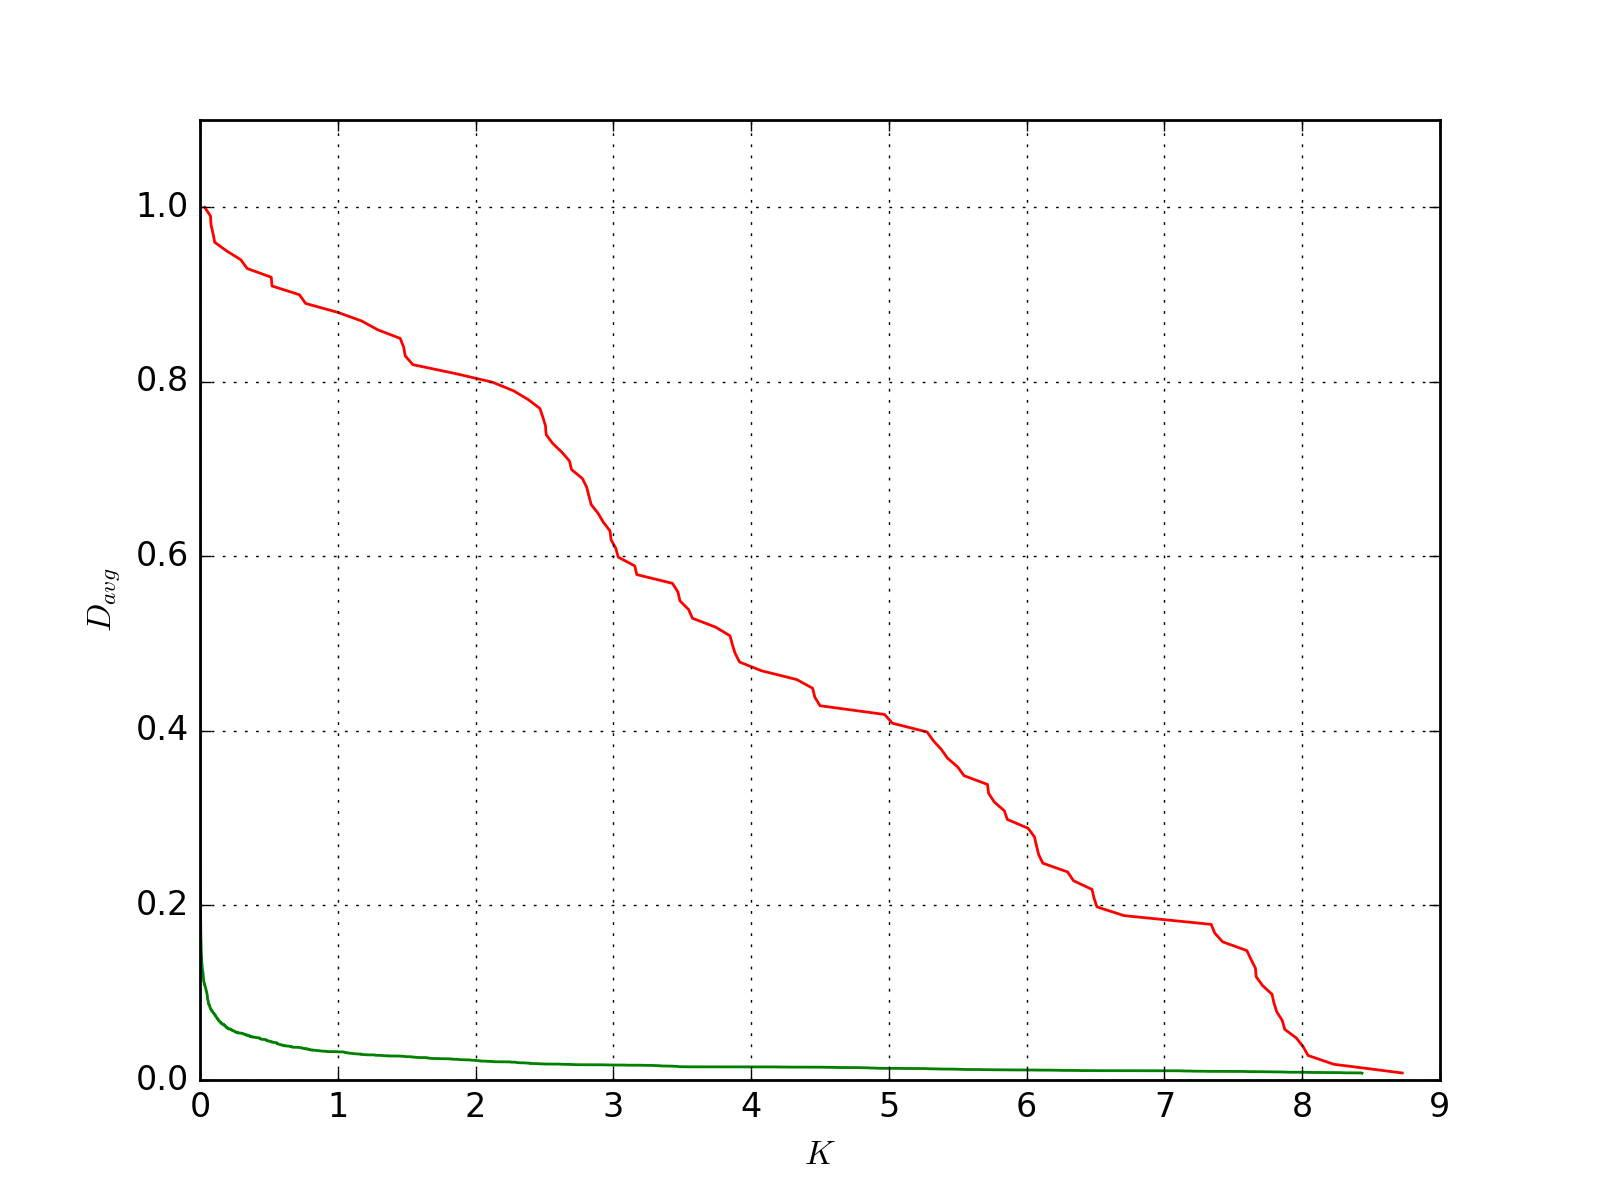
\includegraphics[width=1.0\linewidth]{fig5a.jpg} \\ (a)}
\end{minipage}
\hfill
\begin{minipage}{0.5\linewidth}
\center{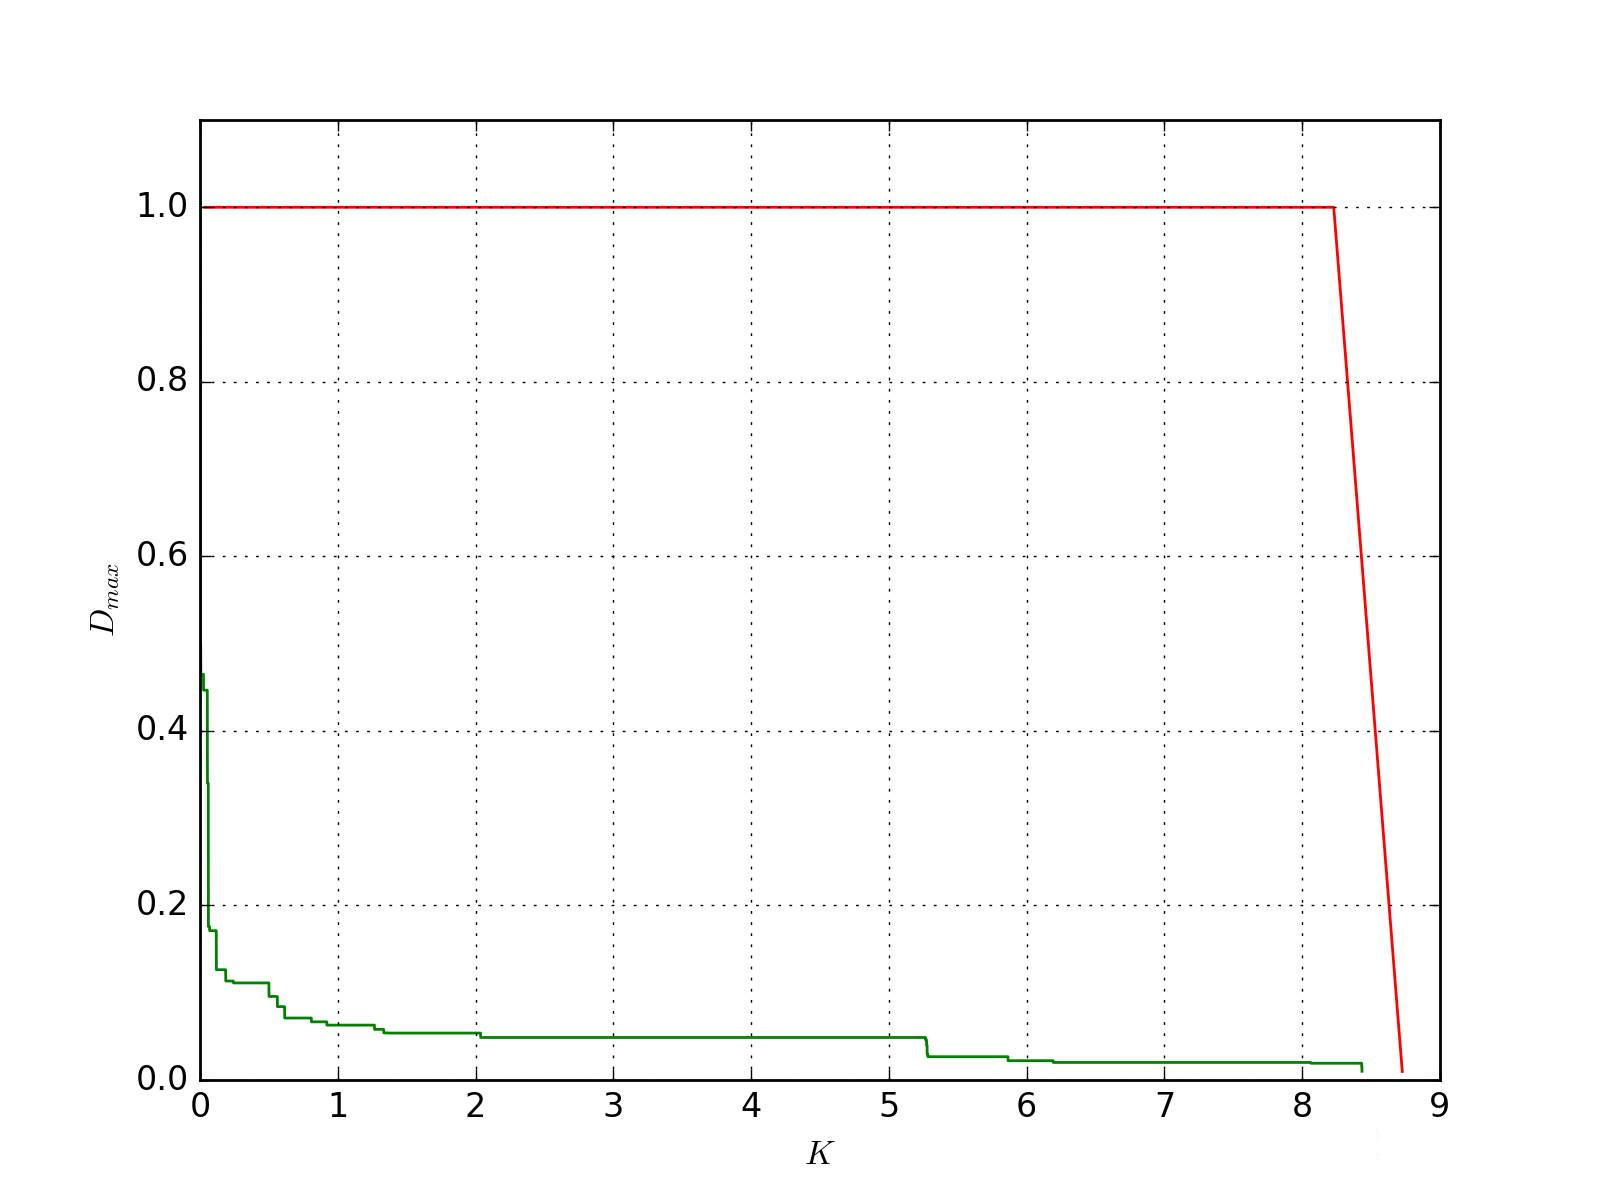
\includegraphics[width=1.0\linewidth]{fig5b.jpg} \\ (b)}
\end{minipage}
\caption{Average (a) and maximum (b) deviation of the current approximation from the exact solution for the parallel algorithm; the number of threads $p = 8$.}
\label{fig_last3}
\end{figure}


\begin{figure}
\begin{minipage}{0.5\linewidth}
\center{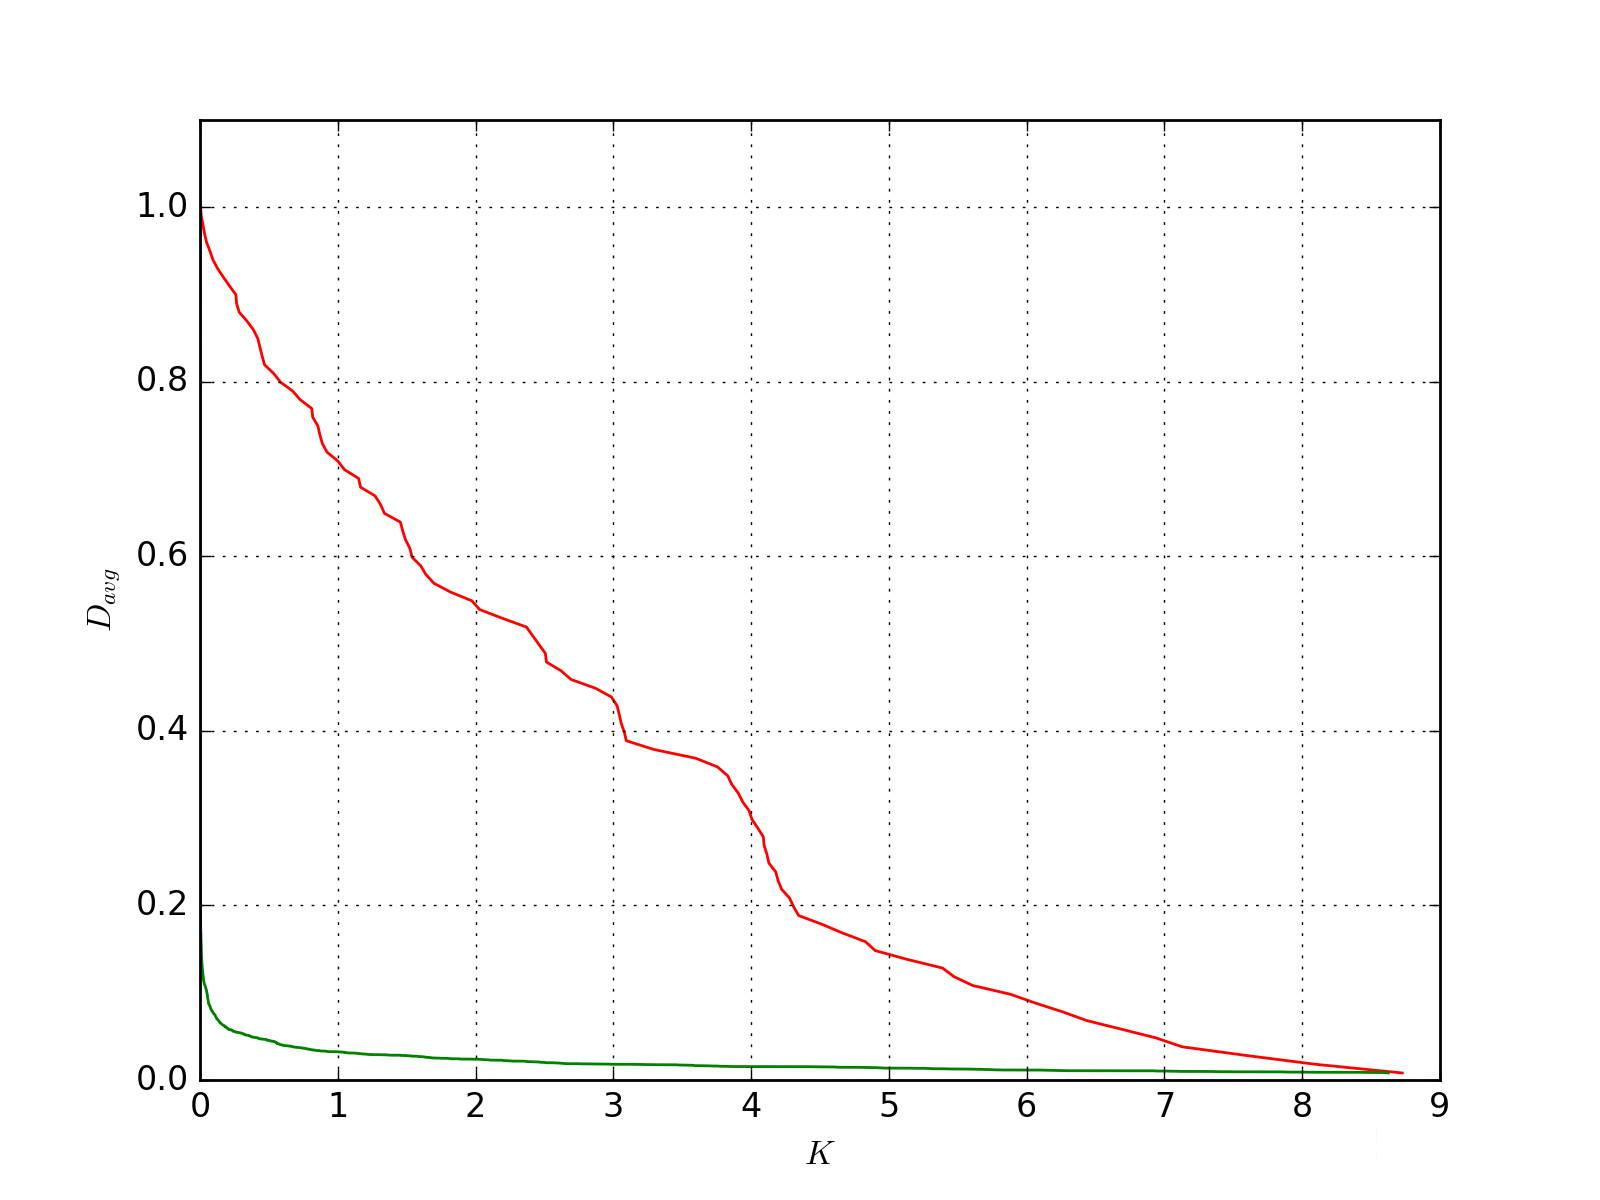
\includegraphics[width=1.0\linewidth]{fig6a.jpg} \\ (a)}
\end{minipage}
\hfill
\begin{minipage}{0.5\linewidth}
\center{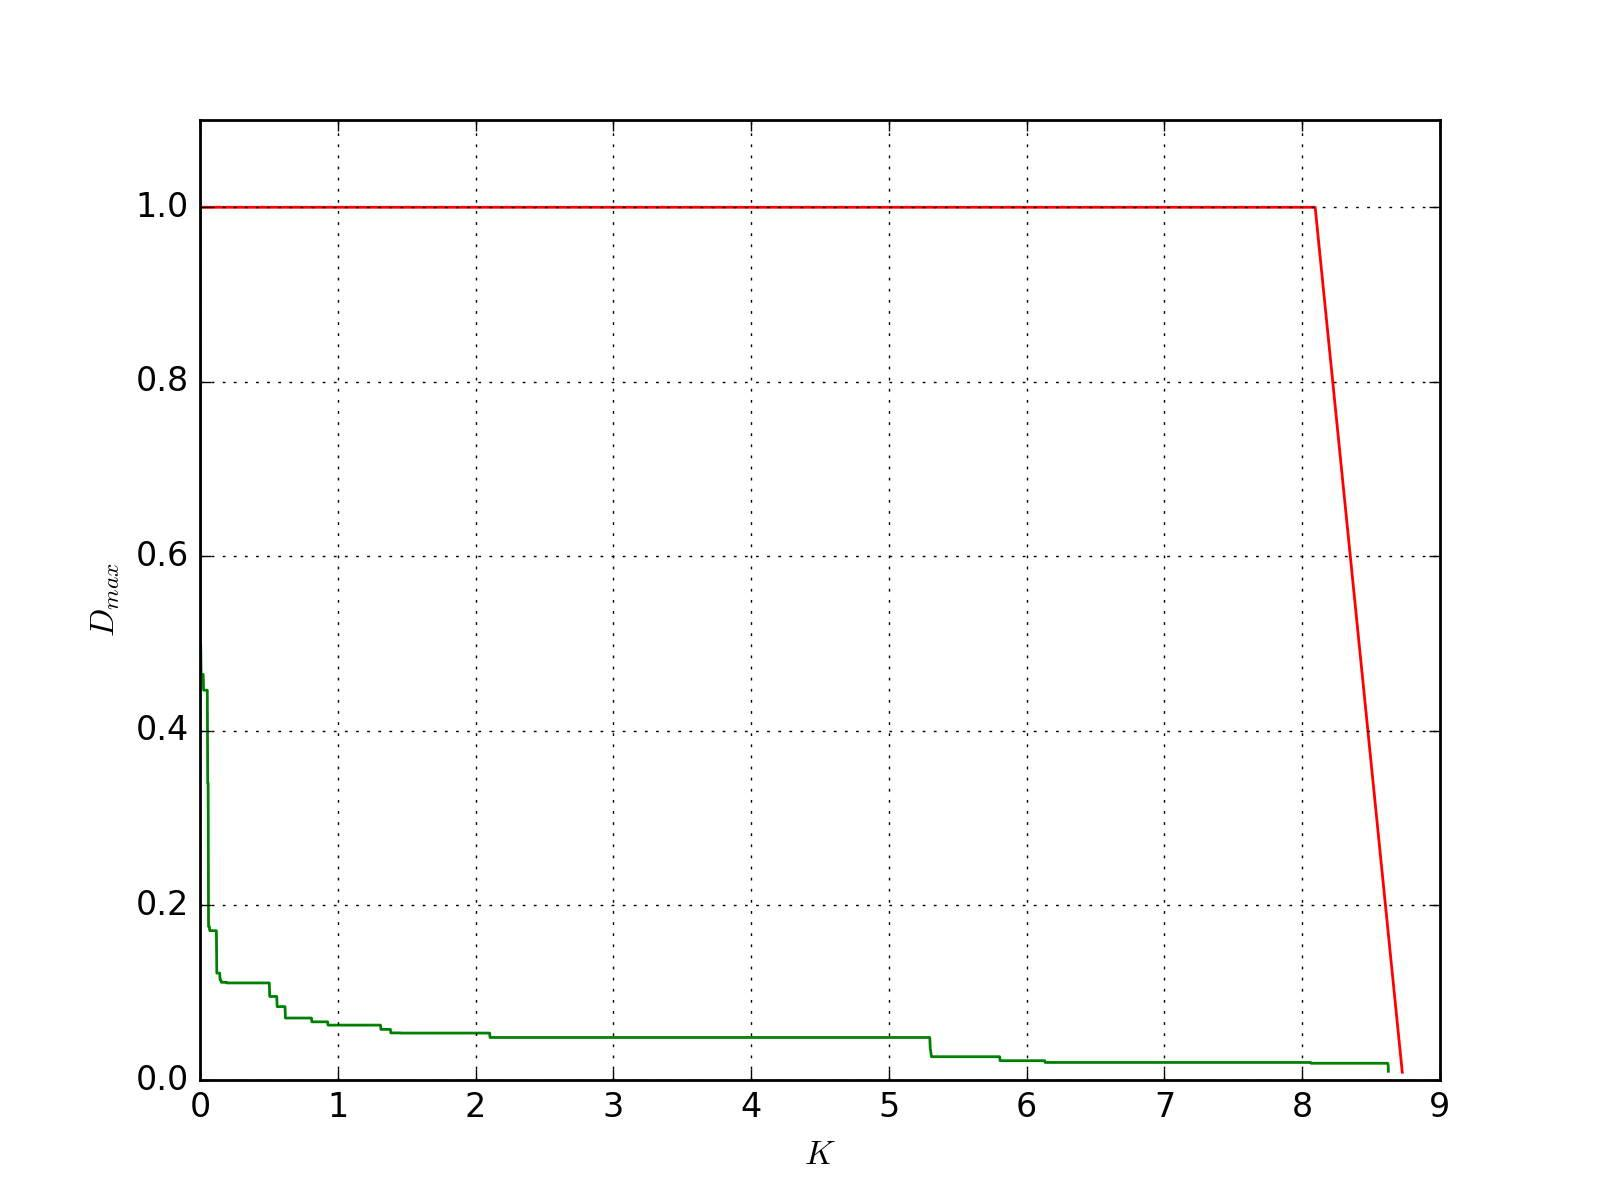
\includegraphics[width=1.0\linewidth]{fig6b.jpg} \\ (b)}
\end{minipage}
\caption{Average (a) and maximum (b) deviation of the current approximation from the exact solution for the parallel algorithm; the number of threads $p = 24$.}
\label{fig_last4}
\end{figure}



The plots clearly demonstrate the uniform convergence to the solutions of the problems of the series when using Scheme 2. The arrangement of curves in Figs.~\ref{fig_last1},~\ref{fig_last2},~\ref{fig_last3} and \ref{fig_last4} demonstrates that when simultaneously solving the problems, one can obtain a good approximation to the solution in all problems within $100 000$ trials (on average as well as in the worst case). In both cases the scheme of problem distribution between the independent threads is inferior to the scheme for simultaneous solving of all problems.

%new text begins

Previous experiments were carried out with the objective functions of the same structure. To demonstrate the uniform convergence for objective functions of a different structure let us consider two mixed series of two-dimensional problems: 50 functions from GKLS \textit{Simple} or \textit{Hard} classes and 50 functions of the form
\begin{eqnarray} \nonumber \label{vagris}
\varphi(y)= -&\left\{\left(\sum^{7}_{i=1}\sum^{7}_{j=1}A_{ij}g_{ij}(y)+B_{ij}h_{ij}(y)\right)^2+\right. \\
&\left.\left(\sum^{7}_{i=1}\sum^{7}_{j=1}C_{ij}g_{ij}(y)+D_{ij}h_{ij}(y)\right)^2\right\}^{1/2},\\ \nonumber
\end{eqnarray}
where
\begin{eqnarray} \nonumber
& y=(y_1,y_2)\in R^2, 0 \leq y_1,y_2 \leq 1, \\ \nonumber
& g_{ij}(y)=\sin(i\pi y_1)\sin(j\pi y_2),  \\ \nonumber
& h_{ij}(y)=\cos(i\pi y_1)\cos(j\pi y_2), \nonumber 
\end{eqnarray}
and coefficients $A_{ij}, B_{ij}, C_{ij}, D_{ij}$  are taken uniformly in the interval $[-1,1]$. The problems with odd numbers are from GKLS classes and the problems with even numbers are based on functions (\ref{vagris}).

Each series of problems was solved using a scheme for distributing the problems between the parallel threads ($S1$) and using the scheme for solving all problems simultaneously ($S2$). The number of employed parallel threads $p$ was varied from 1 to 16. The average numbers of trials executed by the algorithm depending on the number of threads when solving mixed classes of problems are presented in Table \ref{tab:3}.

\begin{table}
	\caption{Average number of iterations for the mixed series of problems}
	\label{tab:3}
	\center
	\begin{tabular}{cccccc}
		\hline\noalign{\smallskip}
		$p$ & \multicolumn{2}{c}{ GKLS \textit{Simple} and (\ref{vagris}) } & & \multicolumn{2}{c}{GKLS \textit{Hard} and (\ref{vagris})} \\
		\noalign{\smallskip} \cline{2-3} \cline{5-6} \noalign{\smallskip}
		 & $S1$ & $S2$ & & $S1$ & $S2$ \\
		\noalign{\smallskip} \hline \noalign{\smallskip}
1	&	234	&	234	&	&	472	&	472	\\
2	&	234	&	240	&	&	472	&	476	\\
4	&	234	&	248	&	&	472	&	469	\\
8	&	234	&	249	&	&	472	&	482	\\
16	&	234	&	251	&	&	472	&	479	\\
		\noalign{\smallskip}\hline
	\end{tabular}
\end{table}


Figs. \ref{fig_last5}, \ref{fig_last6}, \ref{fig_last7} show the functions $D_{av}(K)$ and $D_{max}(K)$ plotted when solving mixed problem series using the sequential algorithm and the parallel algorithm. The number of trials is plotted on the abscissa (in thousands) against the deviation of the current approximation from the exact solution of the problem on the ordinate. The red curve shows the first scheme of problem distributions while the green curve represents the second scheme.

\begin{figure}
\begin{minipage}{0.5\linewidth}
\center{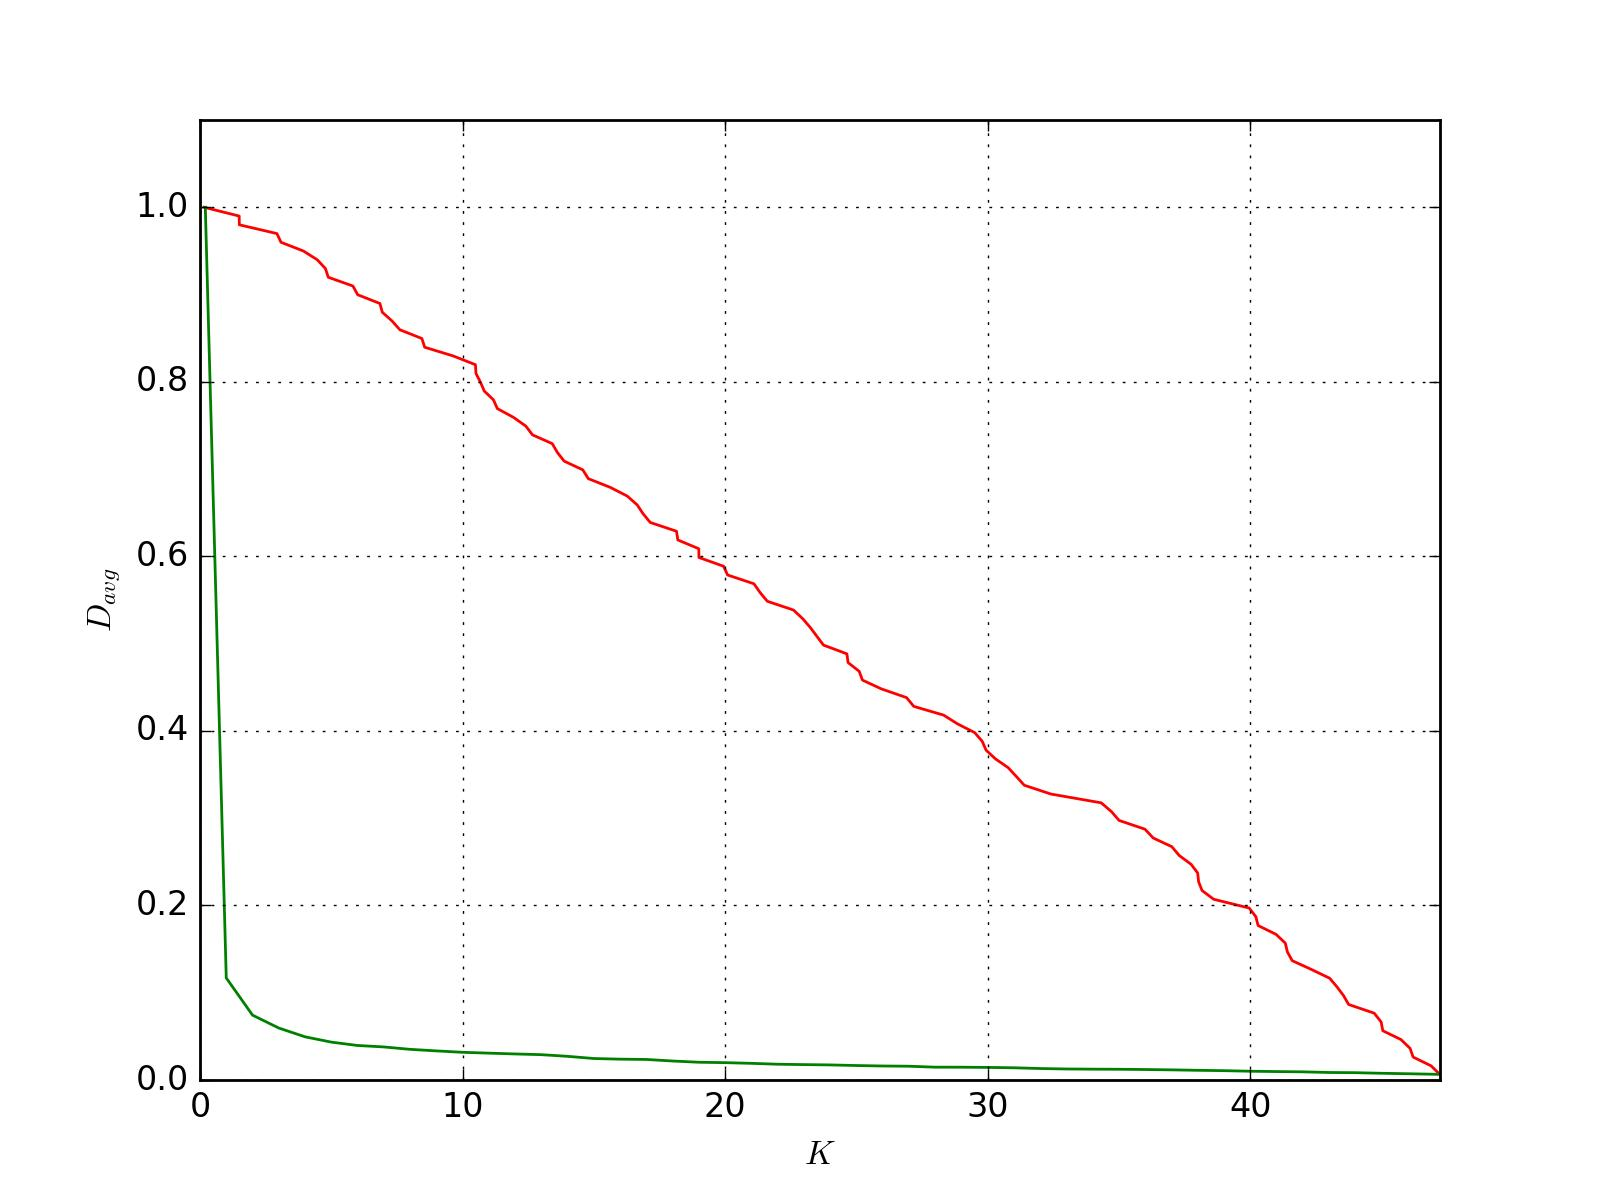
\includegraphics[width=1.0\linewidth]{fig7a.jpg} \\ (a)}
\end{minipage}
\hfill
\begin{minipage}{0.5\linewidth}
\center{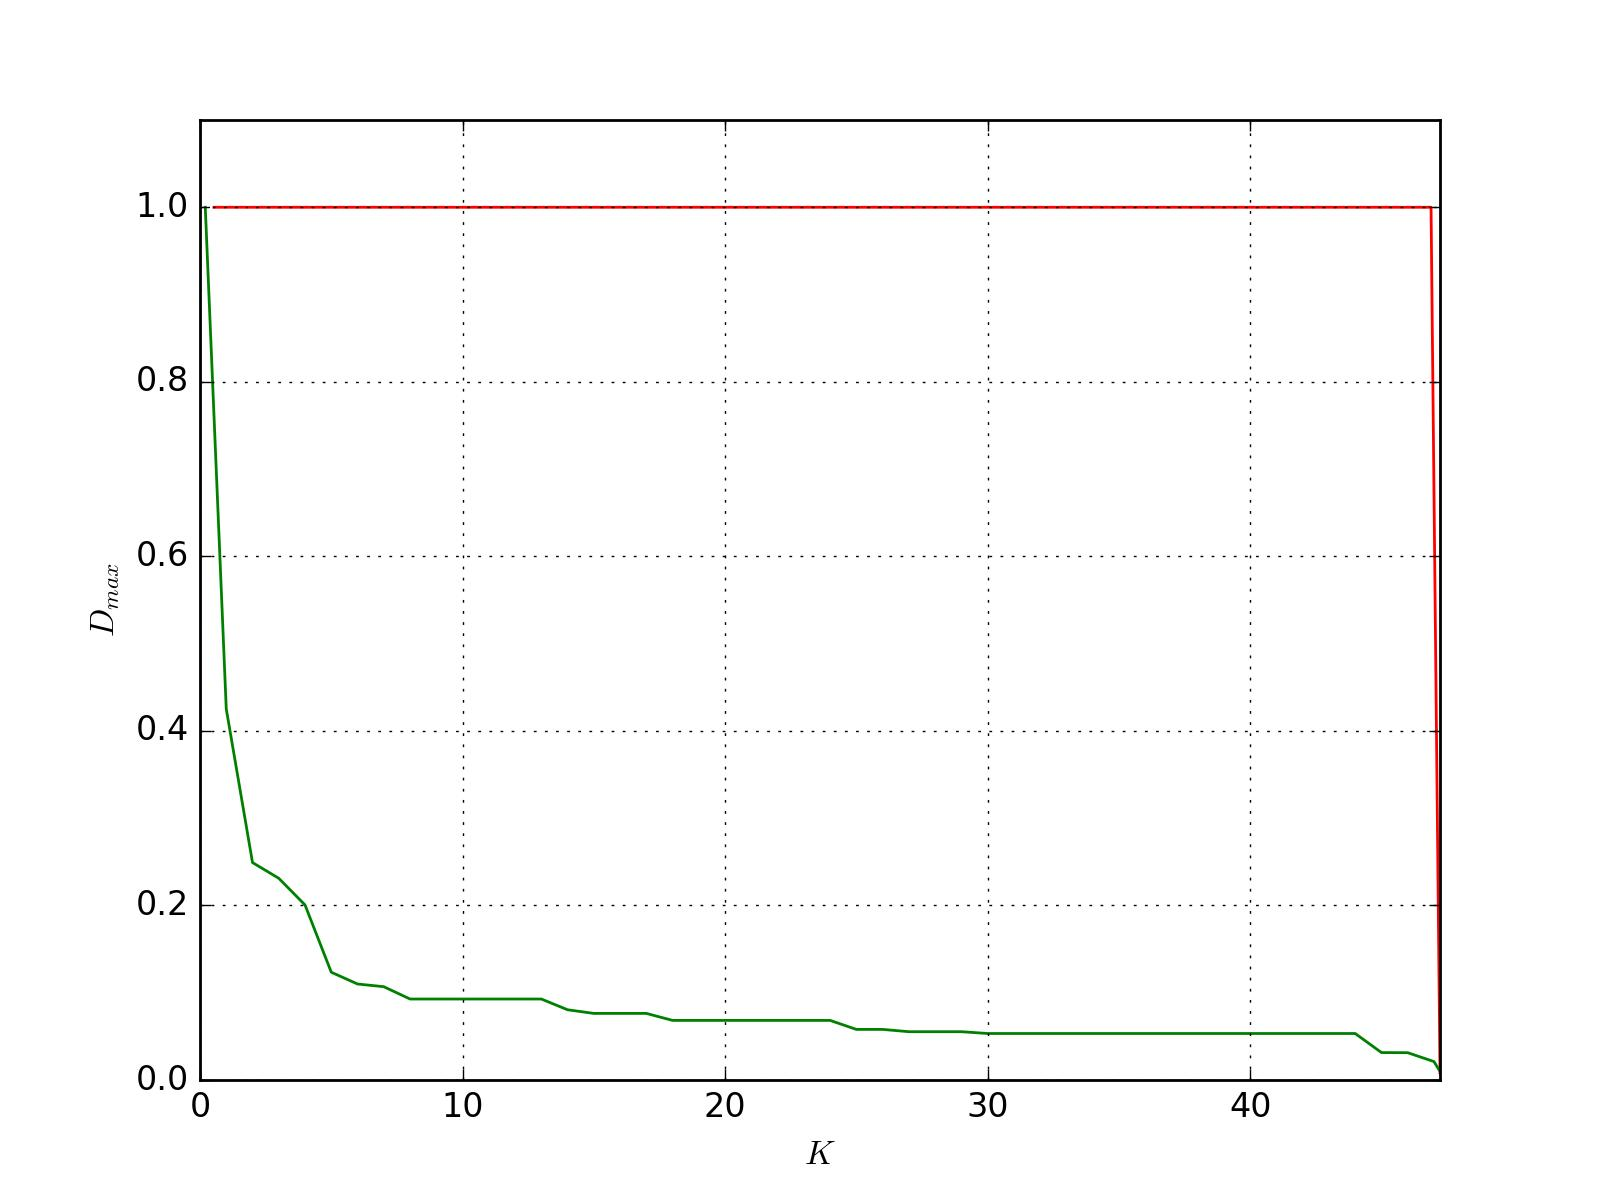
\includegraphics[width=1.0\linewidth]{fig7b.jpg} \\ (b)}
\end{minipage}
\caption{Average (a) and maximum (b) deviation of the current approximation from the exact solution for the sequential algorithm when solving mixed series of problems.}
\label{fig_last5}
\end{figure}

\begin{figure}
\begin{minipage}{0.5\linewidth}
\center{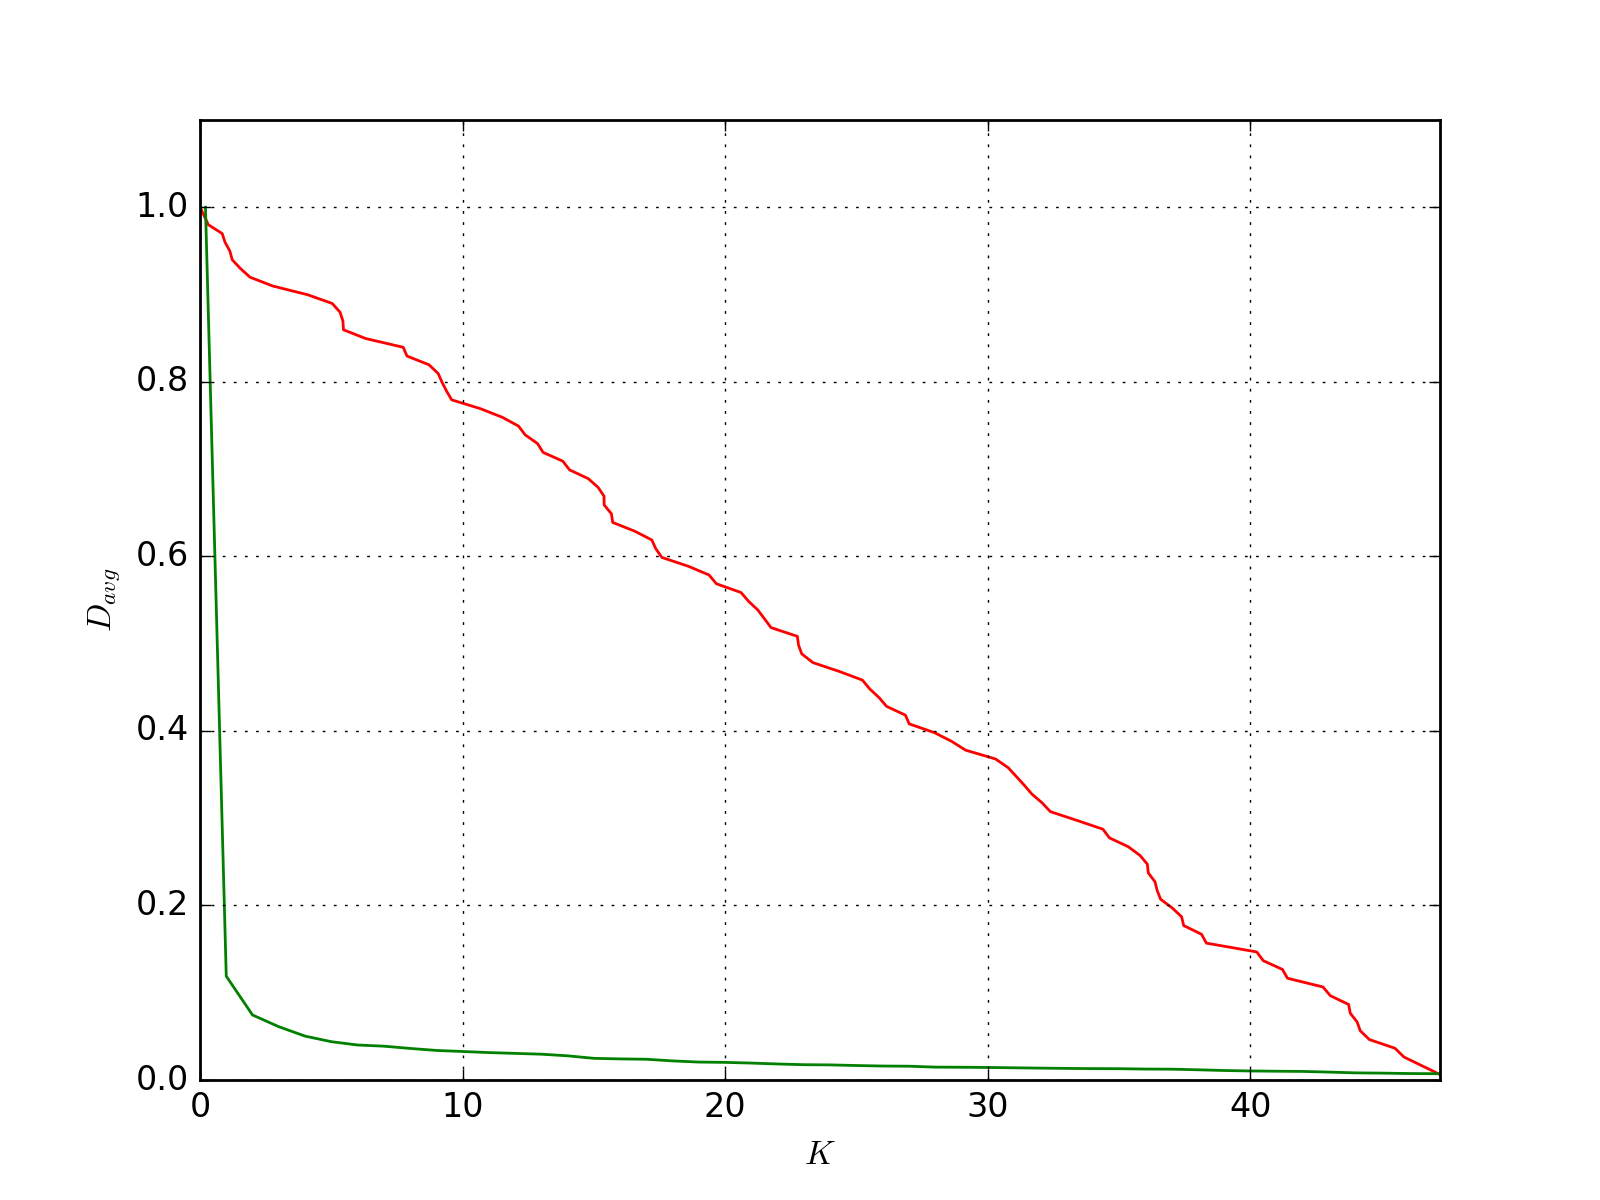
\includegraphics[width=1.0\linewidth]{fig8a.jpg} \\ (a)}
\end{minipage}
\hfill
\begin{minipage}{0.5\linewidth}
\center{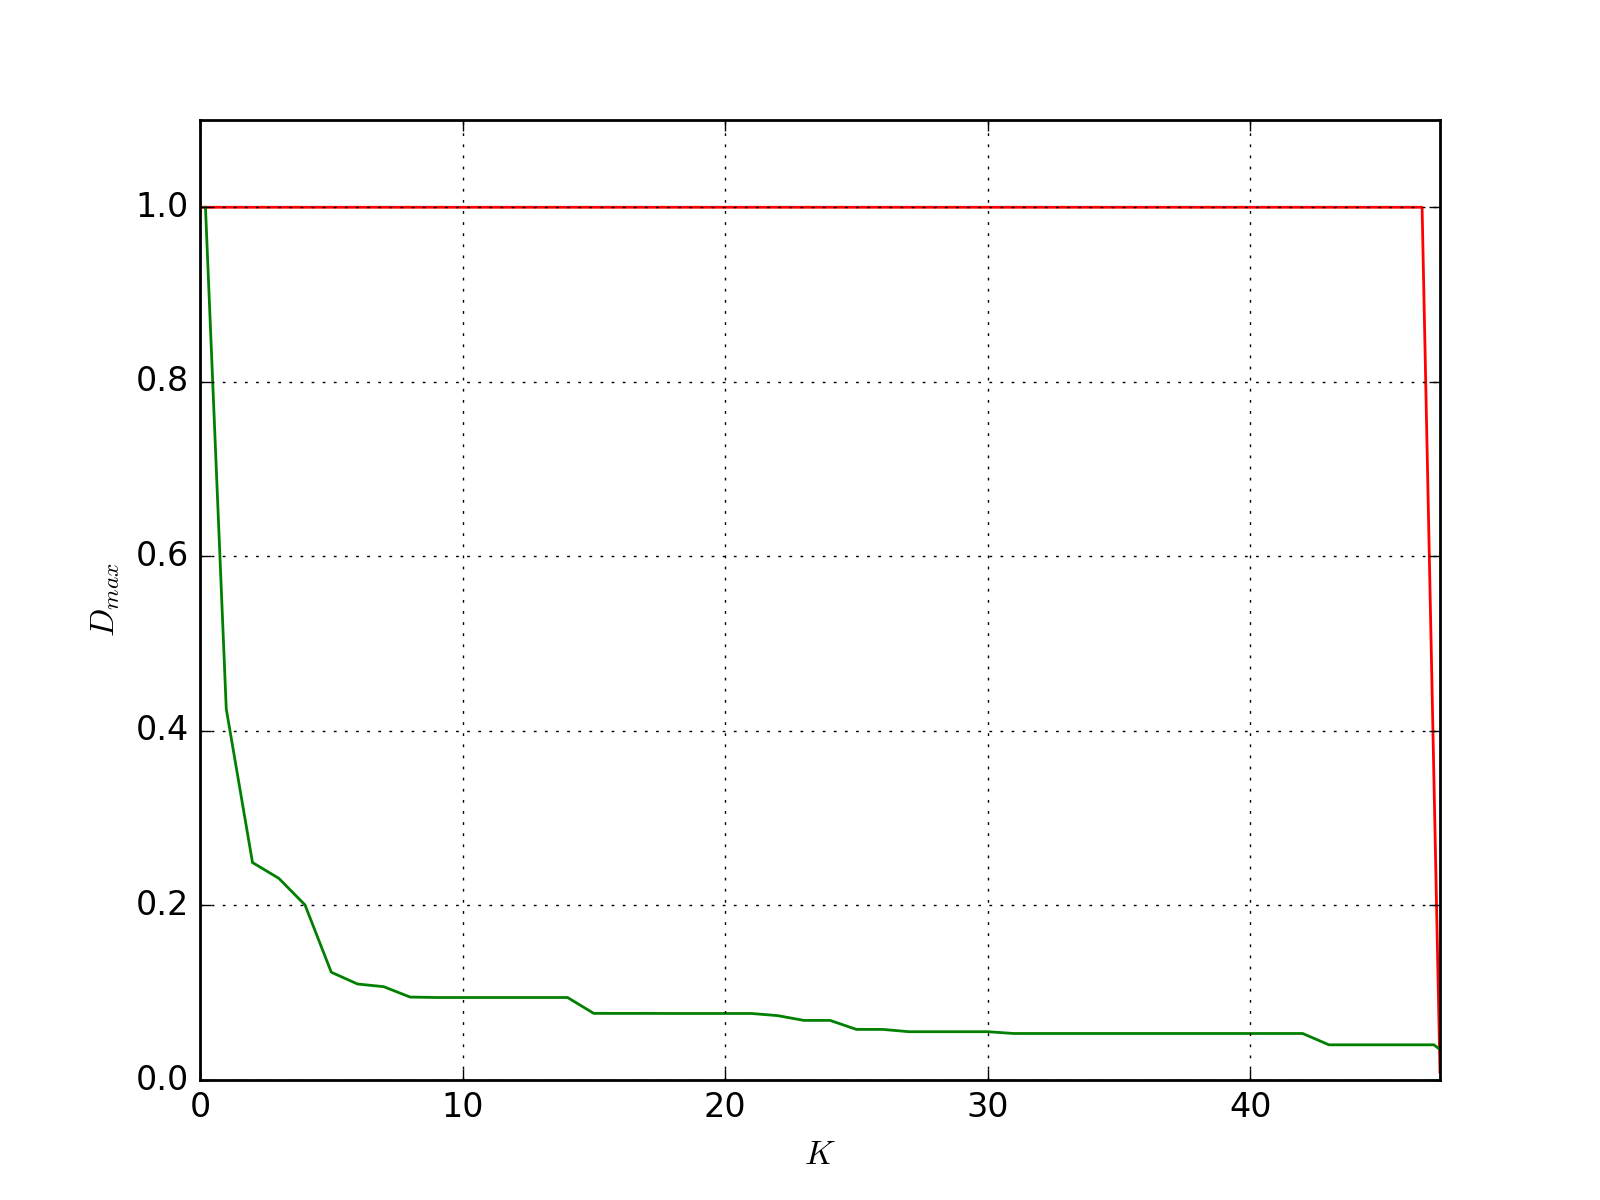
\includegraphics[width=1.0\linewidth]{fig8b.jpg} \\ (b)}
\end{minipage}
\caption{Average (a) and maximum (b) deviation of the current approximation from the exact solution for the parallel algorithm when solving mixed series of problems; the number of threads $p = 8$.}
\label{fig_last6}
\end{figure}

\begin{figure}
\begin{minipage}{0.5\linewidth}
\center{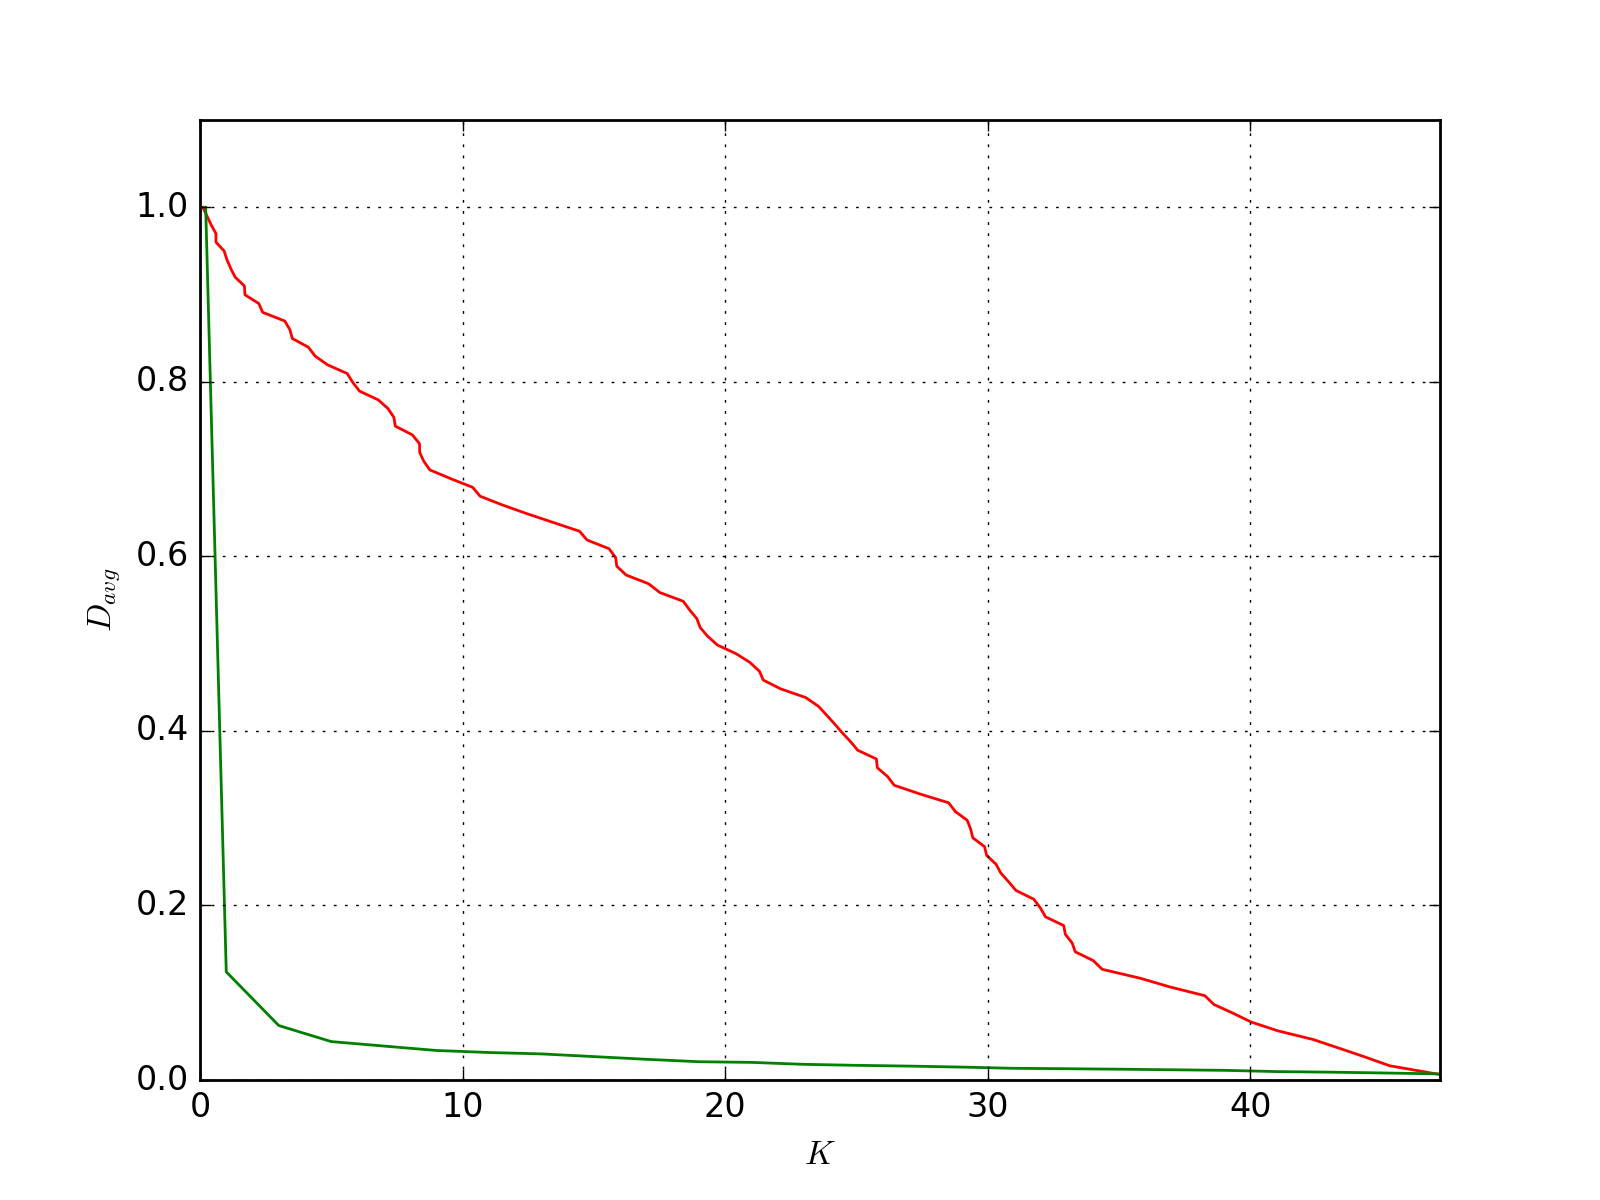
\includegraphics[width=1.0\linewidth]{fig9a.jpg} \\ (a)}
\end{minipage}
\hfill
\begin{minipage}{0.5\linewidth}
\center{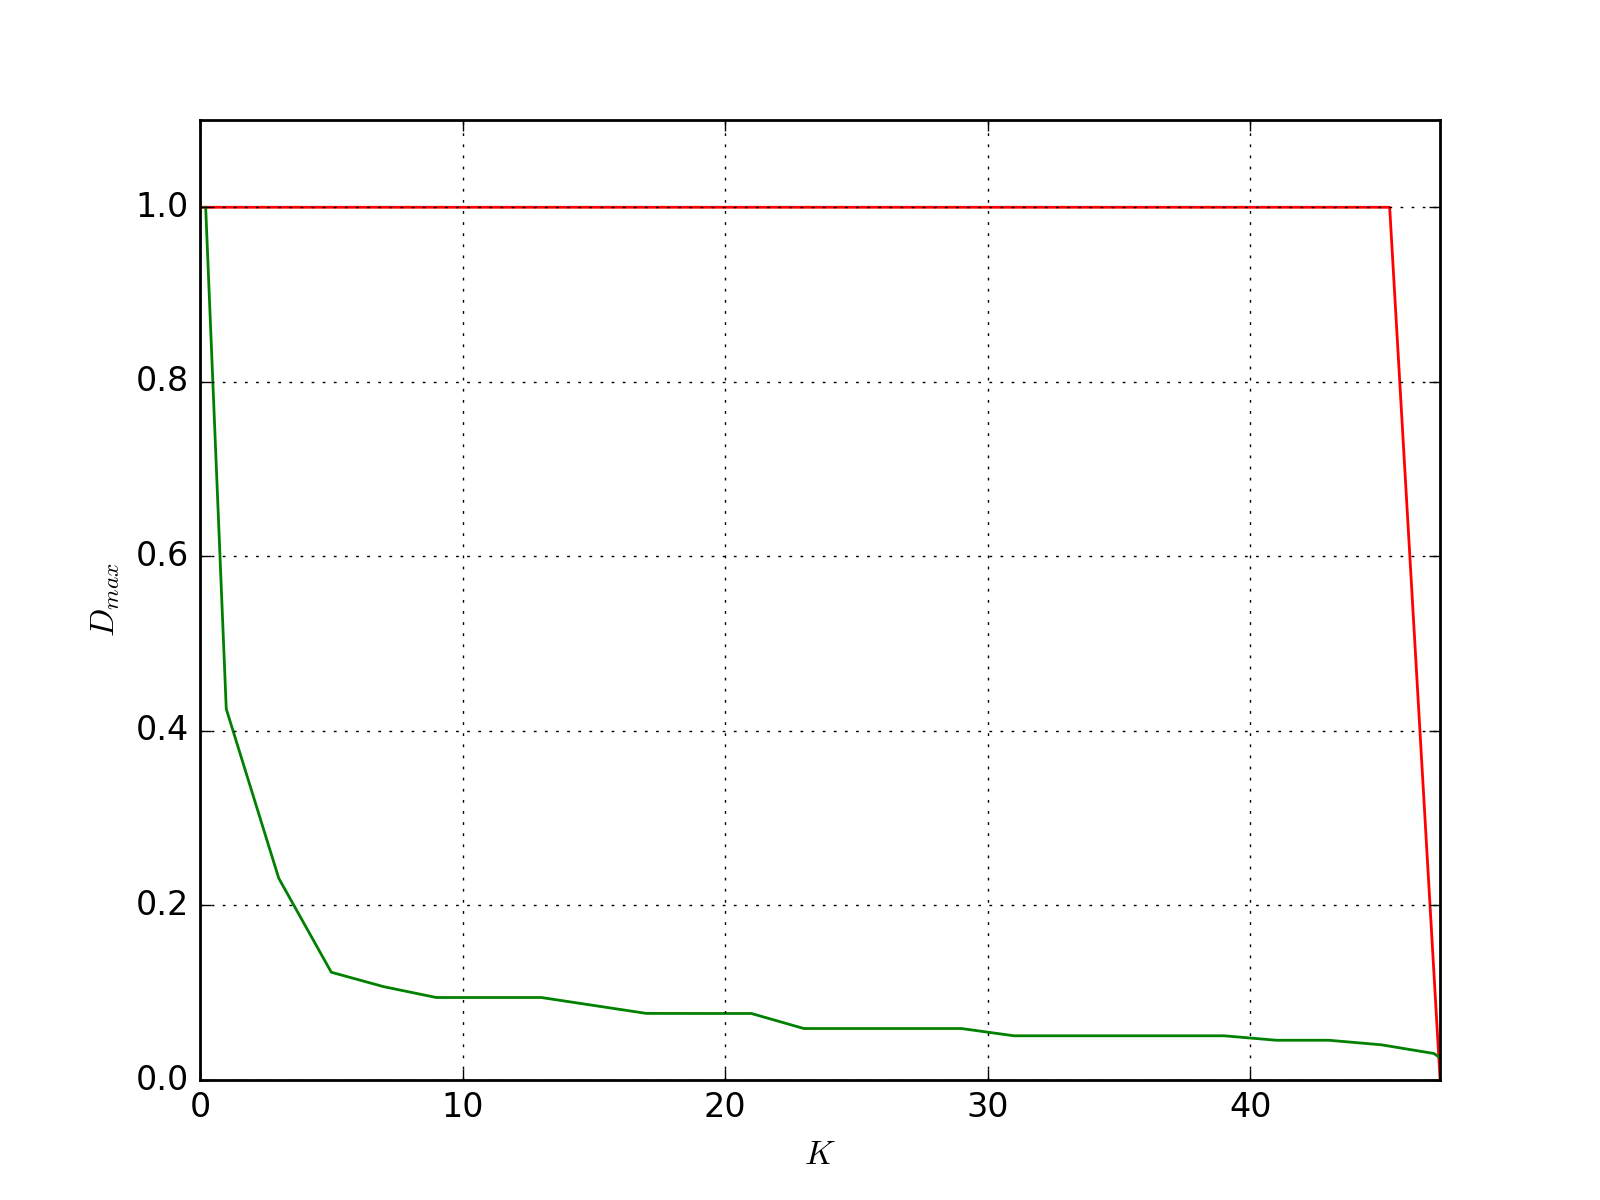
\includegraphics[width=1.0\linewidth]{fig9b.jpg} \\ (b)}
\end{minipage}
\caption{Average (a) and maximum (b) deviation of the current approximation from the exact solution for the parallel algorithm when solving mixed series of problems; the number of threads $p = 16$.}
\label{fig_last7}
\end{figure}

As in the case of objective functions of the same structure, the results show the uniform convergence when using the scheme for solving all problems simultaneously.

%new text ends

The computational experiments were carried out on one of the nodes of a high-performance cluster at Lobachevsky State University of Nizhny Novgorod. The cluster node included 2 Intel Sandy Bridge E5-2660 2.2 GHz CPUs and 64 Gb RAM. The CPU had 8 cores, i.e. a total of 16 physical cores and 16 virtual cores in the hyper-threading mode were available in the node. MS Visual Studio 15 was used to implement the algorithm.

\section{Conclusions }

In this paper, the results obtained when investigating the issues in solving a series of optimization problems are presented. A series of problems may arise when solving a more complex type of problem, for example, a multiple-criteria optimization problem or a larger dimensional one. A modification of the Global Search Algorithm has been proposed to allow several problems to be solved at once and, correspondingly, simultaneously obtain estimates for the solutions to these problems. The theorem regarding the uniform convergence of the novel algorithm has been proven. The computational experiments on a series of several hundred test problems of various dimensions have been carried out. The experiments have clearly demonstrated the uniform convergence.

%Further generalization of the proposed approach onto a wider class of the parallel characteristical algorithms of global optimization \cite{Grishagin1997} seems promising. It would expand its sphere of application essentially since many well-known global optimization algorithms can be represented in the characteristical form. 

% Non-BibTeX users please use
\begin{thebibliography}{}

\bibitem{Strongin2000}
Strongin, R.G., Sergeyev, Ya.D.: Global Optimization with Non-Convex Constraints. Sequential and Parallel Algorithms. Kluwer Academic Publishers, Dordrecht (2000)

\bibitem{Sergeyev2013}
Sergeyev, Ya.D., Strongin, R.G., Lera, D.: Introduction to Global Optimization Exploiting Space-Filling Curves. Springer (2013)

\bibitem{Pinter1996}
Pinter, J. D.: Global Optimization in Action (Continuous and Lipschitz Optimization: Algorithms, Implementations and Applications). Kluwer Academic Publishers, Dordrecht (1996)

\bibitem{Jones2001}
Jones, D. R.: The direct global optimization algorithm. In: Floudas, C. A., Pardalos, P. M. (eds.) The Encyclopedia of Optimization, Second Edition. pp. 725--735. Springer (2009)

\bibitem{Evtushenko2013}
Evtushenko, Y. G., Posypkin, M. A.: A deterministic approach to global box-constrained optimization. Optim. Lett. 7(4), 819--829 (2013)

\bibitem{Zilinskas2008}
Zilinskas, J.: Branch and bound with simplicial partitions for global optimization. Mathematical Modelling and Analysis 13(1), 145--159 (2008)

\bibitem{Zilinskas2010}
Paulavicius, R., Zilinskas, J., Grothey, A.: Investigation of selection strategies in branch and bound algorithm with simplicial partitions and combination of Lipschitz bounds. Optim. Lett. 4(2), 173–--83 (2010)

\bibitem{Sergeyev2000}
Kvasov, D.E., Pizzuti, C., Sergeyev, Y.D.: Local tuning and partition strategies for diagonal GO methods. Numer. Math. 94(1), 93--106 (2003)

\bibitem{Sergeyev2006}
Sergeyev, Ya.D., Kvasov, D.E.: Global search based on efficient diagonal partitions and a set of Lipschitz constants. SIAM J. Optim. 16(3), 910--937 (2006)

\bibitem{Paulavicius2014}
Paulavicius, R., Sergeyev, Y.D., Kvasov, D.E., Zilinskas, J. Globally-biased \textsc{Disimpl} algorithm for expensive global optimization. J. Glob. Optim. 59(2), 545--567 (2014)

\bibitem{Gergel2005}
Gergel, V.P., Strongin, R.G.: Parallel computing for globally optimal decision making on cluster systems. Future Gener. Comput. Syst., 21(5), 673--678 (2005)

\bibitem{Evtushenko2009}
Evtushenko, Yu.G., Malkova, V.U., Stanevichyus, A.A.: Parallel global optimization of functions of several variables. Comput. Math. Math. Phys. 49(2), 246--260 (2009)

\bibitem{He2008}
He, J., Verstak, A., Watson, L.T., Sosonkina, M.: Design and implementation of a massively parallel version of DIRECT. Comput. Optim. Appl. 40(2), 217--245 (2008)

\bibitem{Paulavicius2011}
Paulavicius, R., Zilinskas, J., Grothey, A.: Parallel branch and bound for global optimization with combination of Lipschitz bounds. Optim. Methods Softw. 26(3), 487--498, (2011)

\bibitem{Ehrgott2005}
Ehrgott, M.: Multicriteria Optimization. Springer-Verlag, Berlin Heidelberg (2005)

\bibitem{Sergeyev1994}
Sergeyev, Y. D., Grishagin, V. A. Sequential and parallel algorithms for global optimization. Optim. Methods Softw. 3, 111--124 (1994)

\bibitem{Grishagin1997}
Grishagin, V.A., Sergeyev, Ya.D., Strongin, R.G.: Parallel characteristical algorithms for solving problems of global optimization. J. Glob. Optim. 10(2), 185--206 (1997)

\bibitem{Sergeyev2001}
Sergeyev, Y.D., Famularo D., Pugliese P. Index Branch-and-Bound Algorithm for Lipschitz univariate global optimization with multiextremal constraints. J. Glob. Optim. 21(3), 317--341 (2001) 

\bibitem{Barkalov2002}
Barkalov, K.A., Strongin, R.G.: A global optimization technique with an adaptive order of checking for constraints. Comput. Math. Math. Phys. 42(9), 1289--1300 (2002)

\bibitem{Strongin2003}
Strongin, R.G., Sergeyev, Ya.D.: Global optimization: fractal approach and non-redundant parallelism. J. Glob. Optim. 27(1), 25--50 (2003)

\bibitem{Barkalov2014}
Barkalov, K.A., Gergel, V.P.: Multilevel scheme of dimensionality reduction for parallel global search algorithms. Proceedings of the 1st International Conference on Engineering and Applied Sciences Optimization -- OPT-i 2014, 2111--2124 (2014)

\bibitem{Barkalov2016}
Barkalov, K., Gergel, V.: Parallel global optimization on GPU. J. Glob. Optim. 66(1), 3--20 (2016)

\bibitem{Zilinskas2013}
Zilinskas, A.: On the worst-case optimal multi-objective global optimization. Optim. Lett. 7, 1921--1928 (2013)

\bibitem{Strongin2009}
Strongin, R.G.: Global Optimization Using Space Filling. In: Floudas, C. A., Pardalos, P. M. (eds.) The Encyclopedia of Optimization, Second Edition. pp. 1418-1423. Springer (2009)

\bibitem{Gaviano2003}
Gaviano, M., Lera, D., Kvasov, D.E., Sergeyev, Ya.D.: Software for generation of classes of test functions with known local and global minima for global optimization. ACM Trans. Math. Software 29, 469--480 (2003)


%\bibitem{RefSergeyev2001} Molinaro, A., Pizzuti, C., and Sergeyev, Ya.D.: Acceleration tools for diagonal information global optimization algorithms. Computational Optimization and Applications 18, 5--26 (2001)

%\bibitem{RefGergel1996} Gergel, V.P.: A method of using derivatives in the minimization of multiextremum functions. Computational Mathematics and Mathematical Physics 36(6), 729--742 (1996)

%\bibitem{RefGergel1997} Gergel, V.P.: A global optimization algorithm for multivariate functions with lipschitzian first derivatives. J. Glob. Optim.10(3), 257--281 (1997)

%\bibitem{RefSergeyev1994} Sergeyev, Ya.D., Grishagin, V.A.: A parallel method for finding the global minimum of univariate functions. J. Optim. Theory Appl. 80(3), 513--536 (1994)

%\bibitem{RefSergeyevGrishagin} Sergeyev, Ya.D., Grishagin, V.A.:  Sequential and parallel global optimization algorithms. Optimization Methods and Software. 3, 111--124 (1994)

%\bibitem{RefGergel1999} Gergel, V.P., Sergeyev, Ya.D.: Sequential and parallel algorithms for global minimizing functions with Lipschitzian derivatives. Computers and Mathematics with Applications, 37(4-5), 163--179 (1999)

%\bibitem{RefBarkalov2013} Barkalov, K., Polovinkin, A., Meyerov, I., Sidorov, S., Zolotykh, N.: SVM regression parameters optimization using parallel global search algorithm // Lecture Notes in Computer Science. 7979, 154--166 (2013)

%\bibitem{RefJones} Jones, D.R., Perttunen, C.D., Stuckman, B.E.: Lipschitzian optimization without the lipschitz constant. J. Optim. Theory Appl. 79(1), 157--181 (1993)

%\bibitem{RefGablonsky} Gablonsky, J.M., Kelley, C.T.: A locally-biased form of the DIRECT algorithm. J. Glob. Optim., 21(1), 27--37 (2001)

\end{thebibliography}

\end{document}
% end of file template.tex

